%\chapter{Derivation of two-dimensional PDEs for water waves at random intermediate depths}
\chapter{Derivation of a two-dimensional PDE for water waves at varying water depths}
\label{chap:pde_derivation}

In this appendix, I will present a new \idx{two-dimensional} \index{dimensionality!two|see{two-dimensional}} \PDE in the \idxs{spatial}{domain}, describing the \qidxs{time evolution of}{surface waves} for intermediate, mildly varying water depths. The equation could efficiently be solved with a \idx{time complexity} of $O(N)$\indexs{big O}{notation} per \idx{time step}, where $N$ is the number of \idxsp{surface}{grid point}{s}, using the \CFMM \citep{White1994}. It has not been solved numerically so its behaviour is unknown.

The equation is derived from the \idx{dispersion relation} that is obtained in \idx{Airy wave theory}, namely:

\begin{equation} \label{eq:dispersion}
\omega^2(k) = \left(g\,+\,\frac{\gamma}{\rho}\,k^2\right)\,k\,\tanh(k\,h),
\end{equation}

where $k$ is the \idx{wavenumber} of one \idx{wave component}, $\omega$ is the \idx{angular freequency} of the component, $g$ is the \idxs{gravitational}{acceleration}, $h$ is the \idxs{water}{depth} and $\gamma$ is the \idxs{surface}{tension}. Since this equation describes waves of a single \idx{wavelength}, we can assume that the \idxs{free surface}{elevation} for one wave component can be described by

\begin{equation} \label{eq:component}
\eta(\vec{r},\,t) = A\,e^{i(\vec{k}\cdot\vec{r}\,-\,\omega\,t)},
\end{equation}

where $\eta$ is the free surface elevation, $A$ is the \idxs{wave}{amplitude} and $\vec{k}$ is the wave vector. We make the observation that $k$ and $\vec{k}$ is related to each other by

\begin{equation} \label{eq:kvectok}
k = \left|\vec{k}\right|.
\end{equation}

Although \eqref{eq:component} describes the time evolution of all wave components, it includes variables from the \idxs{frequency}{domain} ($\vec{k}$ and $\omega$ -- note that $k$ depends on $\vec{k}$ according to \eqref{eq:kvectok}), which are not available when working purely in the spatial domain. Furthermore, the equation is indirectly dependent on $h$ and assumes that this variable has the same value on all locations, which may not be the case. We therefore need a way to express the time evolution of the free surface which does not use frequency domain variables and is roboust even for varying water depths.

By \idxe{differentiation!in time}{differentiating} \eqref{eq:component} in time, we obtain

\begin{equation}
\frac{\partial\eta(\vec{r},\,t)}{\partial t} = -i\,\omega\,A\,e^{i(\vec{k}\cdot\vec{r}\,-\,\omega\,t)},
\end{equation}

where $i$ is the \idxs{imaginary}{unit}. The equation can be rewritten as

\begin{equation}
\frac{\partial}{\partial t}\eta(\vec{r},\,t) = -i\,\omega\,\eta(\vec{r},\,t).
\end{equation}

In a manner inspired by the derivation of the \idxs{Schrödinger}{equation}, such as the derivation in \citep{Bransden2000}, let's define the \idxs{scalar}{operator}

\begin{equation} \label{eq:opomega}
\sop{\omega} = i\frac{\partial}{\partial t}
\end{equation}

and we see that

\begin{equation} \label{eq:opomegaaction}
\sop{\omega}\,\eta = \omega\,\eta
\end{equation}

for a wave component described by \eqref{eq:component}. By taking the \idx{gradient} of \eqref{eq:component}, we obtain

\begin{equation}
\nabla\eta(\vec{r},\,t) = i\,\vec{k}\,A\,e^{i(\vec{k}\cdot\vec{r}\,-\,\omega\,t)}
\end{equation}

which can be written as

\begin{equation}
\nabla\eta(\vec{r},\,t) = i\,\vec{k}\,\eta(\vec{r},\,t).
\end{equation}

Let's define the \idxse{vector}{operator}{vector} and \idxsp{scalar}{operator}{s}

\begin{samepage}
\begin{equation} \label{eq:opkvec}
\vop{k} = -i\,\nabla
\end{equation}

\begin{equation} \label{eq:opk2}
\sop{k^2} = \vop{k}^2 = -\nabla^2
\end{equation}
\end{samepage}

and we see that 

\begin{samepage}
\begin{equation} \label{eq:opkvec1action}
\phantom{and}\quad\vop{k}\,\eta = \vec{k}\,\eta,\quad\text{and}
%\vop{k}\,\eta = \vec{k}\,\eta,
\end{equation}

\begin{equation} \label{eq:opk2action}
\sop{k^2}\,\eta = k^2\,\eta
\end{equation}
\end{samepage}

for a wave component described by \eqref{eq:component}. By mutliplying both sides of \eqref{eq:dispersion} with $\eta$, we obtain

\begin{equation}
\omega^2\,\eta = \left(g\,+\,\frac{\gamma}{\rho}\,k^2\right)\,k\,\tanh(k\,h)\,\eta
\end{equation}

which can be rewritten as

\begin{equation} \label{eq:diffeqbad}
\sop{\omega}^2\,\eta = \left(g\,+\,\frac{\gamma}{\rho}\,\sop{k^2}\right)\,k\,\tanh(k\,h)\,\eta.
\end{equation}

We now have an equation almost free from $\vec{k}$ and $\omega$. However, the factor $k\,\tanh(k\,h)$ persists and is diffucult to turn into an operator free from $\vec{k}$. One solution is to turn this factor into a \idxs{convolution}{filter} which works by calculating the \idx{convolution} between the operand and a \idxs{convolution}{kernel}. However, the kernel proves to be difficult to obtain due to the asymptotically increasing valvue of $k\,\tanh(k\,h)$ as $k\rightarrow\infty$. A possibility is to rewrite \eqref{eq:diffeqbad} into

\begin{equation} \label{eq:diffeqbetter}
\sop{\omega}^2\,\eta = h\,\left(g\,+\,\frac{\gamma}{\rho}\,\sop{k^2}\right)\,\sop{k^2}\,\fdfunc{K}(\vec{k}\,h)\,\eta,
\end{equation}

where

\begin{equation} \label{eq:transkernelofxivec}
\fdfunc{K}(\vec{\xi}) = \begin{cases}
1                                                  , & \quad \vec{\xi} = \vec{0} \\[.5em]
\displaystyle\frac{\tanh(|\vec{\xi}|)}{|\vec{\xi}|}, & \quad \vec{\xi} \neq \vec{0}
\end{cases}\ ,
\end{equation}

a $\fdfunc{\ }$ denotes a function or a variable in the frequency domain and $\vec{\xi}$ is a \idxs{dimensionless}{vector}\index{unitless!see{dimensionless}} in the frequency domain, and turn $\fdfunc{K}(\vec{\xi})$ into a convolution filter. The effect of a \idxs{scalar}{operator} $\sop{C}$ applying the filter on a function described by \eqref{eq:component} would be

\begin{equation} \label{eq:opceffect}
\sop{C}\,\eta(\vec{r},\,t) = \fdfunc{K}(\vec{k}\,h)\,\eta(\vec{r},\,t)
\end{equation}

and since the operator applies a convolution filter, it can be described by

\begin{equation} \label{eq:opcfconvolution}
\sop{C}\,\eta(\vec{r},\,t) = \{f\,*\,\eta\}(\vec{r},\,t),
\end{equation}

where $f$ is the \idxs{convolution}{kernel}. With this new operator, \eqref{eq:diffeqbetter} can be rewritten further into

\begin{equation} \label{eq:diffeqspatial}
\sop{\omega}^2\,\eta = h\,\left(g\,+\,\frac{\gamma}{\rho}\,\sop{k^2}\right)\,\sop{k^2}\,\sop{C}\,\eta.
\end{equation}

which is a \PDE completely free from variables in the frequency domain. Combining \eqref{eq:opceffect} and \eqref{eq:opcfconvolution} yeilds

\begin{equation} \label{eq:fconvolutioneffect}
\{f\,*\,\eta\}(\vec{r},\,t) = \fdfunc{K}(\vec{k}\,h)\,\eta(\vec{r},\,t).
\end{equation}

The \idx{convolution theorem} states that

\begin{equation} \label{eq:convolutiontheorem}
\mathcal{F}\{f\,*\,g\} = \mathcal{F}\{f\}\,\cdot\,\mathcal{F}\{g\},
\end{equation}

where $\mathcal{F}$ denotes the \idxs{non-uniform}{Fourier transform} and $\cdot$ denotes point-wise multiplication. By Fourier transforming \eqref{eq:fconvolutioneffect} using this theorem, we obtain

\begin{equation}
\mathcal{F}\{f\}(\vec{k})\ \mathcal{F}\{\eta\}(\vec{k},\,t) = \fdfunc{K}(\vec{k}\,h)\ \mathcal{F}\{\eta\}(\vec{k},\,t)
\end{equation}

which can be rewritten as

\begin{equation} \label{eq:ffourier}
\mathcal{F}\{f\}(\vec{k}) = \fdfunc{K}(\vec{k}\,h)
\end{equation}

by calceling out $\mathcal{F}\{\eta\}(\vec{k},\,t)$ on both sides. For scaling of a function with a real, non-zero number $a$, the non-uniform Fourier transform has the following property:

\begin{equation} \label{eq:fourierscaling}
\mathcal{F}\{h\}(\vec{\xi}) = \frac{1}{|a|^d}\,\mathcal{F}\{f\}\left(\frac{\vec{\xi}}{a}\right)
,\quad
h(\vec{x}) = f(a\vec{x})\ \forall\ \vec{x},
\end{equation}

where $\vec{x}$ is a \idxs{dimensionless}{vector} in the \idxs{spatial}{domain}. Let's define the function

\begin{equation} \label{eq:ftokernel}
K(\vec{x}) = h^2\,f(h\,\vec{x}).
\end{equation}

Since we are working in \idxs{two}{dimensions}, we have $d = 2$ the scaling property of the non-uniform Fourier transform (\eqref{eq:fourierscaling}) tells us that

\begin{equation}
\mathcal{F}\{K\}(\vec{\xi}) = h^2\,\frac{1}{|h|^2}\,\mathcal{F}\{f\}\left(\frac{\vec{\xi}}{h}\right)
\end{equation}

which, by using \eqref{eq:ffourier} can be rewritten as

\begin{equation}
\mathcal{F}\{K\}(\vec{\xi}) = \fdfunc{K}(\vec{\xi}).
\end{equation}

$K(\vec{x})$ is obtained by \idxse{reverse}{non-uniform Fourier transform}{reverse Fourier transforming} this equation:

\begin{equation} \label{eq:kernelfour2d}
K(\vec{x})\, = \,\mathcal{F}^{-1}\{\fdfunc{K}(\vec{\xi})\}(\vec{x})\, = \,\frac{1}{(2\,\pi)^2}\iint\fdfunc{K}(\vec{\xi})\,e^{i\,\vec{\xi}\cdot\vec{x}}\,\opd\vec{\xi}
\end{equation}

where $\mathcal{F}^{-1}$ denotes the \idxs{reverse}{non-uniform Fourier transform}. Although it is very difficult (if not impossible) to obtain the reverse Fourier transform of this function analytically, it is possible to \idxe{approximation}{approximate} it numerically and use the approximation in the convolution filter instead.

With no loss of generality, we can pick a \idxs{polar}{coordinate system}\index{system!polar coordinate|see{polar coordinate system}} $(\xi,\,\theta)$ such that the vector $\vec{x}$ lies on the $\theta = 0$ axis. In that case, \eqref{eq:kernelfour2d} can be rewritten as

\begin{equation}
K(\vec{x})\, = \,\frac{1}{(2\,\pi)^2}\int_{\xi=0}^\infty\int_{\theta=0}^{2\,\pi}\fdfunc{K}(\xi, \theta)\,e^{i\,\xi\,x\cos\theta}\,\xi\,\opd\xi\,\opd\theta,
\end{equation}

where $\xi = |\vec{\xi}|$ and $\theta$ is the angle between the $\vec{x}$ and $\vec{\xi}$ vectors. By realizing that $\fdfunc{K}$ is cilcular symmetric, i.e.

\begin{equation}
\fdfunc{K}(\vec{\xi}) = \fdfunc{K}(\xi),
\end{equation}

and that this leads to that $K$ also is cilcular symmetric, i.e.

\begin{equation}
K(\vec{x}) = K(x),
\end{equation}

where $x = |\vec{x}|$, the integral over $\theta$ may be carried out, and the Fourier transform is now written

\begin{equation} \label{eq:fdkerneltokernel}
K(x)\, = \,\frac{1}{2\,\pi}\int_0^\infty\fdfunc{K}(\xi)\,J_0(x\,\xi)\,\xi\,\opd\xi\, = \,\frac{1}{2\,\pi}\,F_0\{\fdfunc{K}\}(x),
\end{equation}

where $J_0$ is the \idxs{zeroth order}{Bessel function of the first kind} and $F_0$ denotes the \idxs{zeroth order}{Hankel transform}, which can be calculated more efficiently than the reverse \idxs{two-dimensional}{Fourier transform}. The corresponding transformation for calculating $\fdfunc{K}$ from $K$ is given by

\begin{equation} \label{eq:kerneltofdkernel}
\fdfunc{K}(\xi) = 2\,\pi\,F_0\{K\}(\xi).
\end{equation}

In this case, since $K(x)$ was found to vanish very quickly as $x\rightarrow\infty$, it was more efficient to solve \eqref{eq:kerneltofdkernel} by guessing a function $K^*$ for $K$ than to calculate $K$ from \eqref{eq:fdkerneltokernel} directly. A function that was found both to be simple and to match $\fdfunc{K}$ sufficiently well when transformed according to \eqref{eq:kerneltofdkernel} was

\begin{equation} \label{eq:empirical}
K^*(x) = \frac{1}{8\,\pi^3\,x\,(1\,+\,x)}\,e^{-x^2/4},
\end{equation}

where $^*$ denotes an \estimate. Note that both $K$, $\fdfunc{K}$ and the arguments they take are \idx{dimensionless}. $K$ is therefore the \idxs{dimensionless}{convolution kernel}.

%TODO: Include plots
%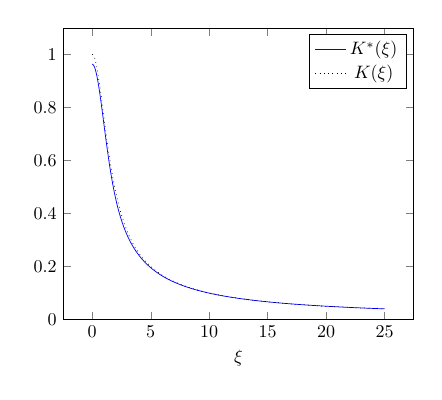
\begin{tikzpicture}[
scale=0.65,]\begin{axis}[
xlabel={$\xi$},
scaled x ticks = false,
x tick label style = {/pgf/number format/fixed},
scaled y ticks = false,
y tick label style = {/pgf/number format/fixed},
ymin=0,
]
\addplot[color=blue,] coordinates {
(0.0000000000, 0.9635604621)
(0.0016000000, 0.9635596998)
(0.0064000000, 0.9635482653)
(0.0144000000, 0.9634987189)
(0.0256000000, 0.9633653491)
(0.0400000000, 0.9630842452)
(0.0576000000, 0.9625734810)
(0.0784000000, 0.9617334882)
(0.1024000000, 0.9604477235)
(0.1296000000, 0.9585837470)
(0.1600000000, 0.9559948463)
(0.1936000000, 0.9525223458)
(0.2304000000, 0.9479987328)
(0.2704000000, 0.9422517168)
(0.3136000000, 0.9351092925)
(0.3600000000, 0.9264058216)
(0.4096000000, 0.9159890558)
(0.4624000000, 0.9037279205)
(0.5184000000, 0.8895207424)
(0.5776000000, 0.8733034744)
(0.6400000000, 0.8550573353)
(0.7056000000, 0.8348151802)
(0.7744000000, 0.8126658679)
(0.8464000000, 0.7887559174)
(0.9216000000, 0.7632878685)
(1.0000000000, 0.7365149937)
(1.0816000000, 0.7087323380)
(1.1664000000, 0.6802644628)
(1.2544000000, 0.6514506898)
(1.3456000000, 0.6226290138)
(1.4400000000, 0.5941201062)
(1.5376000000, 0.5662129045)
(1.6384000000, 0.5391531333)
(1.7424000000, 0.5131357549)
(1.8496000000, 0.4883018299)
(1.9600000000, 0.4647396902)
(2.0736000000, 0.4424897865)
(2.1904000000, 0.4215521748)
(2.3104000000, 0.4018954136)
(2.4336000000, 0.3834656773)
(2.5600000000, 0.3661951117)
(2.6896000000, 0.3500087888)
(2.8224000000, 0.3348299774)
(2.9584000000, 0.3205837538)
(3.0976000000, 0.3071991843)
(3.2400000000, 0.2946104165)
(3.3856000000, 0.2827570205)
(3.5344000000, 0.2715838770)
(3.6864000000, 0.2610408277)
(3.8416000000, 0.2510822324)
(4.0000000000, 0.2416665146)
(4.1616000000, 0.2327557340)
(4.3264000000, 0.2243152041)
(4.4944000000, 0.2163131534)
(4.6656000000, 0.2087204292)
(4.8400000000, 0.2015102374)
(5.0176000000, 0.1946579142)
(5.1984000000, 0.1881407237)
(5.3824000000, 0.1819376793)
(5.5696000000, 0.1760293843)
(5.7600000000, 0.1703978899)
(5.9536000000, 0.1650265679)
(6.1504000000, 0.1598999966)
(6.3504000000, 0.1550038584)
(6.5536000000, 0.1503248471)
(6.7600000000, 0.1458505842)
(6.9696000000, 0.1415695438)
(7.1824000000, 0.1374709837)
(7.3984000000, 0.1335448833)
(7.6176000000, 0.1297818873)
(7.8400000000, 0.1261732538)
(8.0656000000, 0.1227108079)
(8.2944000000, 0.1193868986)
(8.5264000000, 0.1161943597)
(8.7616000000, 0.1131264740)
(9.0000000000, 0.1101769407)
(9.2416000000, 0.1073398450)
(9.4864000000, 0.1046096309)
(9.7344000000, 0.1019810754)
(9.9856000000, 0.0994492658)
(10.2400000000, 0.0970095777)
(10.4976000000, 0.0946576553)
(10.7584000000, 0.0923893936)
(11.0224000000, 0.0902009210)
(11.2896000000, 0.0880885842)
(11.5600000000, 0.0860489338)
(11.8336000000, 0.0840787106)
(12.1104000000, 0.0821748338)
(12.3904000000, 0.0803343893)
(12.6736000000, 0.0785546193)
(12.9600000000, 0.0768329125)
(13.2496000000, 0.0751667946)
(13.5424000000, 0.0735539206)
(13.8384000000, 0.0719920661)
(14.1376000000, 0.0704791207)
(14.4400000000, 0.0690130805)
(14.7456000000, 0.0675920425)
(15.0544000000, 0.0662141979)
(15.3664000000, 0.0648778273)
(15.6816000000, 0.0635812950)
(16.0000000000, 0.0623230446)
(16.3216000000, 0.0611015940)
(16.6464000000, 0.0599155318)
(16.9744000000, 0.0587635129)
(17.3056000000, 0.0576442550)
(17.6400000000, 0.0565565352)
(17.9776000000, 0.0554987984)
(18.3184000000, 0.0544710955)
(18.6624000000, 0.0534714947)
(19.0096000000, 0.0524984789)
(19.3600000000, 0.0515519664)
(19.7136000000, 0.0506310883)
(20.0704000000, 0.0497338895)
(20.4304000000, 0.0488612575)
(20.7936000000, 0.0480100148)
(21.1600000000, 0.0471802286)
(21.5296000000, 0.0463750438)
(21.9024000000, 0.0455870445)
(22.2784000000, 0.0448186421)
(22.6576000000, 0.0440719472)
(23.0400000000, 0.0433420224)
(23.4256000000, 0.0426298354)
(23.8144000000, 0.0419367494)
(24.2064000000, 0.0412581118)
(24.6016000000, 0.0405976096)
(25.0000000000, 0.0399526932)
};
\addlegendentry{$\fdfunc{K}^*(\xi)$}
\addplot[dotted,color=black,] coordinates {
(0.0000000000, 1.0000000000)
(0.0016000000, 0.9999991467)
(0.0064000000, 0.9999863469)
(0.0144000000, 0.9999308857)
(0.0256000000, 0.9997816039)
(0.0400000000, 0.9994670078)
(0.0576000000, 0.9988955457)
(0.0784000000, 0.9979561715)
(0.1024000000, 0.9965193449)
(0.1296000000, 0.9944386408)
(0.1600000000, 0.9915531519)
(0.1936000000, 0.9876908572)
(0.2304000000, 0.9826731008)
(0.2704000000, 0.9763202551)
(0.3136000000, 0.9684585454)
(0.3600000000, 0.9589278726)
(0.4096000000, 0.9475903122)
(0.4624000000, 0.9343387908)
(0.5184000000, 0.9191052939)
(0.5776000000, 0.9018678534)
(0.6400000000, 0.8826555513)
(0.7056000000, 0.8615508678)
(0.7744000000, 0.8386889126)
(0.8464000000, 0.8142533845)
(0.9216000000, 0.7884694584)
(1.0000000000, 0.7615941560)
(1.0816000000, 0.7339050304)
(1.1664000000, 0.7056881595)
(1.2544000000, 0.6772264584)
(1.3456000000, 0.6487892014)
(1.4400000000, 0.6206234217)
(1.5376000000, 0.5929475792)
(1.6384000000, 0.5659476096)
(1.7424000000, 0.5397752241)
(1.8496000000, 0.5145481569)
(1.9600000000, 0.4903519545)
(2.0736000000, 0.4672428669)
(2.1904000000, 0.4452514202)
(2.3104000000, 0.4243863059)
(2.4336000000, 0.4046382957)
(2.5600000000, 0.3859839670)
(2.6896000000, 0.3683890978)
(2.8224000000, 0.3518116516)
(2.9584000000, 0.3362043203)
(3.0976000000, 0.3215166287)
(3.2400000000, 0.3076966286)
(3.3856000000, 0.2946922225)
(3.5344000000, 0.2824521673)
(3.6864000000, 0.2709268052)
(3.8416000000, 0.2600685720)
(4.0000000000, 0.2498323249)
(4.1616000000, 0.2401755293)
(4.3264000000, 0.2310583364)
(4.4944000000, 0.2224435813)
(4.6656000000, 0.2142967215)
(4.8400000000, 0.2065857365)
(5.0176000000, 0.1992809998)
(5.1984000000, 0.1923551365)
(5.3824000000, 0.1857828738)
(5.5696000000, 0.1795408894)
(5.7600000000, 0.1736076634)
(5.9536000000, 0.1679633359)
(6.1504000000, 0.1625895720)
(6.3504000000, 0.1574694354)
(6.5536000000, 0.1525872709)
(6.7600000000, 0.1479285965)
(6.9696000000, 0.1434800035)
(7.1824000000, 0.1392290662)
(7.3984000000, 0.1351642585)
(7.6176000000, 0.1312748788)
(7.8400000000, 0.1275509809)
(8.0656000000, 0.1239833122)
(8.2944000000, 0.1205632565)
(8.5264000000, 0.1172827831)
(8.7616000000, 0.1141343991)
(9.0000000000, 0.1111111077)
(9.2416000000, 0.1082063692)
(9.4864000000, 0.1054140652)
(9.7344000000, 0.1027284674)
(9.9856000000, 0.1001442072)
(10.2400000000, 0.0976562498)
(10.4976000000, 0.0952598688)
(10.7584000000, 0.0929506245)
(11.0224000000, 0.0907243431)
(11.2896000000, 0.0885770975)
(11.5600000000, 0.0865051903)
(11.8336000000, 0.0845051379)
(12.1104000000, 0.0825736557)
(12.3904000000, 0.0807076446)
(12.6736000000, 0.0789041788)
(12.9600000000, 0.0771604938)
(13.2496000000, 0.0754739766)
(13.5424000000, 0.0738421550)
(13.8384000000, 0.0722626893)
(14.1376000000, 0.0707333635)
(14.4400000000, 0.0692520776)
(14.7456000000, 0.0678168403)
(15.0544000000, 0.0664257626)
(15.3664000000, 0.0650770512)
(15.6816000000, 0.0637690032)
(16.0000000000, 0.0625000000)
(16.3216000000, 0.0612685031)
(16.6464000000, 0.0600730488)
(16.9744000000, 0.0589122443)
(17.3056000000, 0.0577847633)
(17.6400000000, 0.0566893424)
(17.9776000000, 0.0556247775)
(18.3184000000, 0.0545899205)
(18.6624000000, 0.0535836763)
(19.0096000000, 0.0526049996)
(19.3600000000, 0.0516528926)
(19.7136000000, 0.0507264021)
(20.0704000000, 0.0498246173)
(20.4304000000, 0.0489466677)
(20.7936000000, 0.0480917205)
(21.1600000000, 0.0472589792)
(21.5296000000, 0.0464476813)
(21.9024000000, 0.0456570969)
(22.2784000000, 0.0448865269)
(22.6576000000, 0.0441353012)
(23.0400000000, 0.0434027778)
(23.4256000000, 0.0426883410)
(23.8144000000, 0.0419914002)
(24.2064000000, 0.0413113887)
(24.6016000000, 0.0406477627)
(25.0000000000, 0.0400000000)
};
\addlegendentry{$\fdfunc{K}(\xi)$}
\end{axis}\end{tikzpicture}

%% Title: glps_renderer figure
% Creator: GL2PS 1.3.6, (C) 1999-2011 C. Geuzaine
% For: Octave
% CreationDate: Wed Jun 13 10:06:23 2012
\begin{pgfpicture}
{
\pgftransformshift{\pgfpoint{246.399994pt}{73.195633pt}}
\pgfnode{rectangle}{north}{\fontsize{10}{0}\selectfont\textcolor[rgb]{0,0,0}{{10}}}{}{\pgfusepath{discard}}}
{
\pgftransformshift{\pgfpoint{333.199982pt}{73.195633pt}}
\pgfnode{rectangle}{north}{\fontsize{10}{0}\selectfont\textcolor[rgb]{0,0,0}{{15}}}{}{\pgfusepath{discard}}}
{
\pgftransformshift{\pgfpoint{419.999969pt}{73.195633pt}}
\pgfnode{rectangle}{north}{\fontsize{10}{0}\selectfont\textcolor[rgb]{0,0,0}{{20}}}{}{\pgfusepath{discard}}}
{
\pgftransformshift{\pgfpoint{506.799957pt}{73.195633pt}}
\pgfnode{rectangle}{north}{\fontsize{10}{0}\selectfont\textcolor[rgb]{0,0,0}{{25}}}{}{\pgfusepath{discard}}}
{
\pgftransformshift{\pgfpoint{67.799995pt}{78.200020pt}}
\pgfnode{rectangle}{east}{\fontsize{10}{0}\selectfont\textcolor[rgb]{0,0,0}{{0}}}{}{\pgfusepath{discard}}}
{
\pgftransformshift{\pgfpoint{67.799995pt}{135.250015pt}}
\pgfnode{rectangle}{east}{\fontsize{10}{0}\selectfont\textcolor[rgb]{0,0,0}{{0.005}}}{}{\pgfusepath{discard}}}
{
\pgftransformshift{\pgfpoint{72.799995pt}{73.195633pt}}
\pgfnode{rectangle}{north}{\fontsize{10}{0}\selectfont\textcolor[rgb]{0,0,0}{{0}}}{}{\pgfusepath{discard}}}
{
\pgftransformshift{\pgfpoint{159.599991pt}{73.195633pt}}
\pgfnode{rectangle}{north}{\fontsize{10}{0}\selectfont\textcolor[rgb]{0,0,0}{{5}}}{}{\pgfusepath{discard}}}
{
\pgftransformshift{\pgfpoint{67.799995pt}{192.300003pt}}
\pgfnode{rectangle}{east}{\fontsize{10}{0}\selectfont\textcolor[rgb]{0,0,0}{{0.01}}}{}{\pgfusepath{discard}}}
{
\pgftransformshift{\pgfpoint{67.799995pt}{249.349991pt}}
\pgfnode{rectangle}{east}{\fontsize{10}{0}\selectfont\textcolor[rgb]{0,0,0}{{0.015}}}{}{\pgfusepath{discard}}}
{
\pgftransformshift{\pgfpoint{67.799995pt}{306.399994pt}}
\pgfnode{rectangle}{east}{\fontsize{10}{0}\selectfont\textcolor[rgb]{0,0,0}{{0.02}}}{}{\pgfusepath{discard}}}
{
\pgftransformshift{\pgfpoint{67.799995pt}{363.449982pt}}
\pgfnode{rectangle}{east}{\fontsize{10}{0}\selectfont\textcolor[rgb]{0,0,0}{{0.025}}}{}{\pgfusepath{discard}}}
{
\pgftransformshift{\pgfpoint{67.799995pt}{420.499969pt}}
\pgfnode{rectangle}{east}{\fontsize{10}{0}\selectfont\textcolor[rgb]{0,0,0}{{0.03}}}{}{\pgfusepath{discard}}}
\color[rgb]{0.000000,0.000000,0.000000}
\pgfsetlinewidth{0.500000pt}
\pgfsetdash{{16pt}{0pt}}{0pt}
\pgfpathmoveto{\pgfpoint{506.750000pt}{420.500000pt}}
\pgflineto{\pgfpoint{72.750000pt}{420.500000pt}}
\pgfusepath{stroke}
\pgfpathmoveto{\pgfpoint{72.750000pt}{420.500000pt}}
\pgflineto{\pgfpoint{72.750000pt}{78.187500pt}}
\pgfusepath{stroke}
\pgfpathmoveto{\pgfpoint{506.750000pt}{420.500000pt}}
\pgflineto{\pgfpoint{506.750000pt}{78.187500pt}}
\pgfusepath{stroke}
\pgfpathmoveto{\pgfpoint{72.750000pt}{85.187500pt}}
\pgflineto{\pgfpoint{72.750000pt}{78.187500pt}}
\pgfusepath{stroke}
\pgfpathmoveto{\pgfpoint{72.750000pt}{413.437500pt}}
\pgflineto{\pgfpoint{72.750000pt}{420.500000pt}}
\pgfusepath{stroke}
\pgfpathmoveto{\pgfpoint{159.562500pt}{85.187500pt}}
\pgflineto{\pgfpoint{159.562500pt}{78.187500pt}}
\pgfusepath{stroke}
\pgfpathmoveto{\pgfpoint{159.562500pt}{413.437500pt}}
\pgflineto{\pgfpoint{159.562500pt}{420.500000pt}}
\pgfusepath{stroke}
\pgfpathmoveto{\pgfpoint{506.750000pt}{78.187500pt}}
\pgflineto{\pgfpoint{72.750000pt}{78.187500pt}}
\pgfusepath{stroke}
\pgfpathmoveto{\pgfpoint{246.375000pt}{85.187500pt}}
\pgflineto{\pgfpoint{246.375000pt}{78.187500pt}}
\pgfusepath{stroke}
\pgfpathmoveto{\pgfpoint{246.375000pt}{413.437500pt}}
\pgflineto{\pgfpoint{246.375000pt}{420.500000pt}}
\pgfusepath{stroke}
\pgfpathmoveto{\pgfpoint{333.187500pt}{85.187500pt}}
\pgflineto{\pgfpoint{333.187500pt}{78.187500pt}}
\pgfusepath{stroke}
\pgfpathmoveto{\pgfpoint{333.187500pt}{413.437500pt}}
\pgflineto{\pgfpoint{333.187500pt}{420.500000pt}}
\pgfusepath{stroke}
\pgfpathmoveto{\pgfpoint{420.000000pt}{85.187500pt}}
\pgflineto{\pgfpoint{420.000000pt}{78.187500pt}}
\pgfusepath{stroke}
\pgfpathmoveto{\pgfpoint{420.000000pt}{413.437500pt}}
\pgflineto{\pgfpoint{420.000000pt}{420.500000pt}}
\pgfusepath{stroke}
\pgfpathmoveto{\pgfpoint{506.750000pt}{85.187500pt}}
\pgflineto{\pgfpoint{506.750000pt}{78.187500pt}}
\pgfusepath{stroke}
\pgfpathmoveto{\pgfpoint{506.750000pt}{413.437500pt}}
\pgflineto{\pgfpoint{506.750000pt}{420.500000pt}}
\pgfusepath{stroke}
\pgfpathmoveto{\pgfpoint{79.750000pt}{78.187500pt}}
\pgflineto{\pgfpoint{72.750000pt}{78.187500pt}}
\pgfusepath{stroke}
\pgfpathmoveto{\pgfpoint{499.750000pt}{78.187500pt}}
\pgflineto{\pgfpoint{506.750000pt}{78.187500pt}}
\pgfusepath{stroke}
\pgfpathmoveto{\pgfpoint{79.750000pt}{135.250000pt}}
\pgflineto{\pgfpoint{72.750000pt}{135.250000pt}}
\pgfusepath{stroke}
\pgfpathmoveto{\pgfpoint{499.750000pt}{135.250000pt}}
\pgflineto{\pgfpoint{506.750000pt}{135.250000pt}}
\pgfusepath{stroke}
\pgfpathmoveto{\pgfpoint{79.750000pt}{192.250000pt}}
\pgflineto{\pgfpoint{72.750000pt}{192.250000pt}}
\pgfusepath{stroke}
\pgfpathmoveto{\pgfpoint{499.750000pt}{192.250000pt}}
\pgflineto{\pgfpoint{506.750000pt}{192.250000pt}}
\pgfusepath{stroke}
\pgfpathmoveto{\pgfpoint{79.750000pt}{249.312500pt}}
\pgflineto{\pgfpoint{72.750000pt}{249.312500pt}}
\pgfusepath{stroke}
\pgfpathmoveto{\pgfpoint{499.750000pt}{249.312500pt}}
\pgflineto{\pgfpoint{506.750000pt}{249.312500pt}}
\pgfusepath{stroke}
\pgfpathmoveto{\pgfpoint{79.750000pt}{306.375000pt}}
\pgflineto{\pgfpoint{72.750000pt}{306.375000pt}}
\pgfusepath{stroke}
\pgfpathmoveto{\pgfpoint{499.750000pt}{306.375000pt}}
\pgflineto{\pgfpoint{506.750000pt}{306.375000pt}}
\pgfusepath{stroke}
\pgfpathmoveto{\pgfpoint{79.750000pt}{363.437500pt}}
\pgflineto{\pgfpoint{72.750000pt}{363.437500pt}}
\pgfusepath{stroke}
\pgfpathmoveto{\pgfpoint{499.750000pt}{363.437500pt}}
\pgflineto{\pgfpoint{506.750000pt}{363.437500pt}}
\pgfusepath{stroke}
\pgfpathmoveto{\pgfpoint{79.750000pt}{420.500000pt}}
\pgflineto{\pgfpoint{72.750000pt}{420.500000pt}}
\pgfusepath{stroke}
\pgfpathmoveto{\pgfpoint{499.750000pt}{420.500000pt}}
\pgflineto{\pgfpoint{506.750000pt}{420.500000pt}}
\pgfusepath{stroke}
\color[rgb]{0.000000,0.000000,1.000000}
\pgfsetdash{}{0pt}
\pgfpathmoveto{\pgfpoint{76.250000pt}{363.375000pt}}
\pgflineto{\pgfpoint{74.500000pt}{366.250000pt}}
\pgfusepath{stroke}
\pgfpathmoveto{\pgfpoint{78.000000pt}{358.812500pt}}
\pgflineto{\pgfpoint{76.250000pt}{363.375000pt}}
\pgfusepath{stroke}
\pgfpathmoveto{\pgfpoint{79.687500pt}{352.687500pt}}
\pgflineto{\pgfpoint{78.000000pt}{358.812500pt}}
\pgfusepath{stroke}
\pgfpathmoveto{\pgfpoint{81.437500pt}{345.312500pt}}
\pgflineto{\pgfpoint{79.687500pt}{352.687500pt}}
\pgfusepath{stroke}
\pgfpathmoveto{\pgfpoint{83.187500pt}{336.875000pt}}
\pgflineto{\pgfpoint{81.437500pt}{345.312500pt}}
\pgfusepath{stroke}
\pgfpathmoveto{\pgfpoint{84.937500pt}{327.687500pt}}
\pgflineto{\pgfpoint{83.187500pt}{336.875000pt}}
\pgfusepath{stroke}
\pgfpathmoveto{\pgfpoint{86.687500pt}{318.062500pt}}
\pgflineto{\pgfpoint{84.937500pt}{327.687500pt}}
\pgfusepath{stroke}
\pgfpathmoveto{\pgfpoint{88.375000pt}{308.187500pt}}
\pgflineto{\pgfpoint{86.687500pt}{318.062500pt}}
\pgfusepath{stroke}
\pgfpathmoveto{\pgfpoint{90.125000pt}{298.312500pt}}
\pgflineto{\pgfpoint{88.375000pt}{308.187500pt}}
\pgfusepath{stroke}
\pgfpathmoveto{\pgfpoint{91.875000pt}{288.500000pt}}
\pgflineto{\pgfpoint{90.125000pt}{298.312500pt}}
\pgfusepath{stroke}
\pgfpathmoveto{\pgfpoint{93.625000pt}{278.937500pt}}
\pgflineto{\pgfpoint{91.875000pt}{288.500000pt}}
\pgfusepath{stroke}
\pgfpathmoveto{\pgfpoint{95.312500pt}{269.750000pt}}
\pgflineto{\pgfpoint{93.625000pt}{278.937500pt}}
\pgfusepath{stroke}
\pgfpathmoveto{\pgfpoint{97.062500pt}{260.937500pt}}
\pgflineto{\pgfpoint{95.312500pt}{269.750000pt}}
\pgfusepath{stroke}
\pgfpathmoveto{\pgfpoint{98.812500pt}{252.562500pt}}
\pgflineto{\pgfpoint{97.062500pt}{260.937500pt}}
\pgfusepath{stroke}
\pgfpathmoveto{\pgfpoint{100.562500pt}{244.687500pt}}
\pgflineto{\pgfpoint{98.812500pt}{252.562500pt}}
\pgfusepath{stroke}
\pgfpathmoveto{\pgfpoint{102.312500pt}{237.187500pt}}
\pgflineto{\pgfpoint{100.562500pt}{244.687500pt}}
\pgfusepath{stroke}
\pgfpathmoveto{\pgfpoint{104.000000pt}{230.187500pt}}
\pgflineto{\pgfpoint{102.312500pt}{237.187500pt}}
\pgfusepath{stroke}
\pgfpathmoveto{\pgfpoint{105.750000pt}{223.625000pt}}
\pgflineto{\pgfpoint{104.000000pt}{230.187500pt}}
\pgfusepath{stroke}
\pgfpathmoveto{\pgfpoint{107.500000pt}{217.500000pt}}
\pgflineto{\pgfpoint{105.750000pt}{223.625000pt}}
\pgfusepath{stroke}
\pgfpathmoveto{\pgfpoint{109.250000pt}{211.750000pt}}
\pgflineto{\pgfpoint{107.500000pt}{217.500000pt}}
\pgfusepath{stroke}
\pgfpathmoveto{\pgfpoint{110.937500pt}{206.375000pt}}
\pgflineto{\pgfpoint{109.250000pt}{211.750000pt}}
\pgfusepath{stroke}
\pgfpathmoveto{\pgfpoint{112.687500pt}{201.312500pt}}
\pgflineto{\pgfpoint{110.937500pt}{206.375000pt}}
\pgfusepath{stroke}
\pgfpathmoveto{\pgfpoint{114.437500pt}{196.625000pt}}
\pgflineto{\pgfpoint{112.687500pt}{201.312500pt}}
\pgfusepath{stroke}
\pgfpathmoveto{\pgfpoint{116.187500pt}{192.250000pt}}
\pgflineto{\pgfpoint{114.437500pt}{196.625000pt}}
\pgfusepath{stroke}
\pgfpathmoveto{\pgfpoint{117.937500pt}{188.125000pt}}
\pgflineto{\pgfpoint{116.187500pt}{192.250000pt}}
\pgfusepath{stroke}
\pgfpathmoveto{\pgfpoint{119.625000pt}{184.250000pt}}
\pgflineto{\pgfpoint{117.937500pt}{188.125000pt}}
\pgfusepath{stroke}
\pgfpathmoveto{\pgfpoint{121.375000pt}{180.625000pt}}
\pgflineto{\pgfpoint{119.625000pt}{184.250000pt}}
\pgfusepath{stroke}
\pgfpathmoveto{\pgfpoint{123.125000pt}{177.250000pt}}
\pgflineto{\pgfpoint{121.375000pt}{180.625000pt}}
\pgfusepath{stroke}
\pgfpathmoveto{\pgfpoint{124.875000pt}{174.062500pt}}
\pgflineto{\pgfpoint{123.125000pt}{177.250000pt}}
\pgfusepath{stroke}
\pgfpathmoveto{\pgfpoint{126.562500pt}{171.000000pt}}
\pgflineto{\pgfpoint{124.875000pt}{174.062500pt}}
\pgfusepath{stroke}
\pgfpathmoveto{\pgfpoint{128.312500pt}{168.187500pt}}
\pgflineto{\pgfpoint{126.562500pt}{171.000000pt}}
\pgfusepath{stroke}
\pgfpathmoveto{\pgfpoint{130.062500pt}{165.500000pt}}
\pgflineto{\pgfpoint{128.312500pt}{168.187500pt}}
\pgfusepath{stroke}
\pgfpathmoveto{\pgfpoint{131.812500pt}{163.000000pt}}
\pgflineto{\pgfpoint{130.062500pt}{165.500000pt}}
\pgfusepath{stroke}
\pgfpathmoveto{\pgfpoint{133.500000pt}{160.625000pt}}
\pgflineto{\pgfpoint{131.812500pt}{163.000000pt}}
\pgfusepath{stroke}
\pgfpathmoveto{\pgfpoint{135.250000pt}{158.312500pt}}
\pgflineto{\pgfpoint{133.500000pt}{160.625000pt}}
\pgfusepath{stroke}
\pgfpathmoveto{\pgfpoint{137.000000pt}{156.187500pt}}
\pgflineto{\pgfpoint{135.250000pt}{158.312500pt}}
\pgfusepath{stroke}
\pgfpathmoveto{\pgfpoint{138.750000pt}{154.125000pt}}
\pgflineto{\pgfpoint{137.000000pt}{156.187500pt}}
\pgfusepath{stroke}
\pgfpathmoveto{\pgfpoint{140.500000pt}{152.187500pt}}
\pgflineto{\pgfpoint{138.750000pt}{154.125000pt}}
\pgfusepath{stroke}
\pgfpathmoveto{\pgfpoint{142.187500pt}{150.375000pt}}
\pgflineto{\pgfpoint{140.500000pt}{152.187500pt}}
\pgfusepath{stroke}
\pgfpathmoveto{\pgfpoint{143.937500pt}{148.625000pt}}
\pgflineto{\pgfpoint{142.187500pt}{150.375000pt}}
\pgfusepath{stroke}
\pgfpathmoveto{\pgfpoint{145.687500pt}{146.937500pt}}
\pgflineto{\pgfpoint{143.937500pt}{148.625000pt}}
\pgfusepath{stroke}
\pgfpathmoveto{\pgfpoint{147.437500pt}{145.375000pt}}
\pgflineto{\pgfpoint{145.687500pt}{146.937500pt}}
\pgfusepath{stroke}
\pgfpathmoveto{\pgfpoint{149.125000pt}{143.812500pt}}
\pgflineto{\pgfpoint{147.437500pt}{145.375000pt}}
\pgfusepath{stroke}
\pgfpathmoveto{\pgfpoint{150.875000pt}{142.375000pt}}
\pgflineto{\pgfpoint{149.125000pt}{143.812500pt}}
\pgfusepath{stroke}
\pgfpathmoveto{\pgfpoint{152.625000pt}{141.000000pt}}
\pgflineto{\pgfpoint{150.875000pt}{142.375000pt}}
\pgfusepath{stroke}
\pgfpathmoveto{\pgfpoint{154.375000pt}{139.625000pt}}
\pgflineto{\pgfpoint{152.625000pt}{141.000000pt}}
\pgfusepath{stroke}
\pgfpathmoveto{\pgfpoint{156.125000pt}{138.375000pt}}
\pgflineto{\pgfpoint{154.375000pt}{139.625000pt}}
\pgfusepath{stroke}
\pgfpathmoveto{\pgfpoint{157.812500pt}{137.125000pt}}
\pgflineto{\pgfpoint{156.125000pt}{138.375000pt}}
\pgfusepath{stroke}
\pgfpathmoveto{\pgfpoint{159.562500pt}{136.000000pt}}
\pgflineto{\pgfpoint{157.812500pt}{137.125000pt}}
\pgfusepath{stroke}
\pgfpathmoveto{\pgfpoint{161.312500pt}{134.812500pt}}
\pgflineto{\pgfpoint{159.562500pt}{136.000000pt}}
\pgfusepath{stroke}
\pgfpathmoveto{\pgfpoint{163.062500pt}{133.750000pt}}
\pgflineto{\pgfpoint{161.312500pt}{134.812500pt}}
\pgfusepath{stroke}
\pgfpathmoveto{\pgfpoint{164.750000pt}{132.687500pt}}
\pgflineto{\pgfpoint{163.062500pt}{133.750000pt}}
\pgfusepath{stroke}
\pgfpathmoveto{\pgfpoint{166.500000pt}{131.687500pt}}
\pgflineto{\pgfpoint{164.750000pt}{132.687500pt}}
\pgfusepath{stroke}
\pgfpathmoveto{\pgfpoint{168.250000pt}{130.687500pt}}
\pgflineto{\pgfpoint{166.500000pt}{131.687500pt}}
\pgfusepath{stroke}
\pgfpathmoveto{\pgfpoint{170.000000pt}{129.750000pt}}
\pgflineto{\pgfpoint{168.250000pt}{130.687500pt}}
\pgfusepath{stroke}
\pgfpathmoveto{\pgfpoint{171.750000pt}{128.875000pt}}
\pgflineto{\pgfpoint{170.000000pt}{129.750000pt}}
\pgfusepath{stroke}
\pgfpathmoveto{\pgfpoint{173.437500pt}{128.000000pt}}
\pgflineto{\pgfpoint{171.750000pt}{128.875000pt}}
\pgfusepath{stroke}
\pgfpathmoveto{\pgfpoint{175.187500pt}{127.125000pt}}
\pgflineto{\pgfpoint{173.437500pt}{128.000000pt}}
\pgfusepath{stroke}
\pgfpathmoveto{\pgfpoint{176.937500pt}{126.312500pt}}
\pgflineto{\pgfpoint{175.187500pt}{127.125000pt}}
\pgfusepath{stroke}
\pgfpathmoveto{\pgfpoint{178.687500pt}{125.562500pt}}
\pgflineto{\pgfpoint{176.937500pt}{126.312500pt}}
\pgfusepath{stroke}
\pgfpathmoveto{\pgfpoint{180.375000pt}{124.812500pt}}
\pgflineto{\pgfpoint{178.687500pt}{125.562500pt}}
\pgfusepath{stroke}
\pgfpathmoveto{\pgfpoint{182.125000pt}{124.062500pt}}
\pgflineto{\pgfpoint{180.375000pt}{124.812500pt}}
\pgfusepath{stroke}
\pgfpathmoveto{\pgfpoint{183.875000pt}{123.312500pt}}
\pgflineto{\pgfpoint{182.125000pt}{124.062500pt}}
\pgfusepath{stroke}
\pgfpathmoveto{\pgfpoint{185.625000pt}{122.625000pt}}
\pgflineto{\pgfpoint{183.875000pt}{123.312500pt}}
\pgfusepath{stroke}
\pgfpathmoveto{\pgfpoint{187.375000pt}{121.937500pt}}
\pgflineto{\pgfpoint{185.625000pt}{122.625000pt}}
\pgfusepath{stroke}
\pgfpathmoveto{\pgfpoint{189.062500pt}{121.312500pt}}
\pgflineto{\pgfpoint{187.375000pt}{121.937500pt}}
\pgfusepath{stroke}
\pgfpathmoveto{\pgfpoint{190.812500pt}{120.687500pt}}
\pgflineto{\pgfpoint{189.062500pt}{121.312500pt}}
\pgfusepath{stroke}
\pgfpathmoveto{\pgfpoint{192.562500pt}{120.062500pt}}
\pgflineto{\pgfpoint{190.812500pt}{120.687500pt}}
\pgfusepath{stroke}
\pgfpathmoveto{\pgfpoint{194.312500pt}{119.437500pt}}
\pgflineto{\pgfpoint{192.562500pt}{120.062500pt}}
\pgfusepath{stroke}
\pgfpathmoveto{\pgfpoint{196.000000pt}{118.875000pt}}
\pgflineto{\pgfpoint{194.312500pt}{119.437500pt}}
\pgfusepath{stroke}
\pgfpathmoveto{\pgfpoint{197.750000pt}{118.312500pt}}
\pgflineto{\pgfpoint{196.000000pt}{118.875000pt}}
\pgfusepath{stroke}
\pgfpathmoveto{\pgfpoint{199.500000pt}{117.750000pt}}
\pgflineto{\pgfpoint{197.750000pt}{118.312500pt}}
\pgfusepath{stroke}
\pgfpathmoveto{\pgfpoint{201.250000pt}{117.250000pt}}
\pgflineto{\pgfpoint{199.500000pt}{117.750000pt}}
\pgfusepath{stroke}
\pgfpathmoveto{\pgfpoint{203.000000pt}{116.687500pt}}
\pgflineto{\pgfpoint{201.250000pt}{117.250000pt}}
\pgfusepath{stroke}
\pgfpathmoveto{\pgfpoint{204.687500pt}{116.187500pt}}
\pgflineto{\pgfpoint{203.000000pt}{116.687500pt}}
\pgfusepath{stroke}
\pgfpathmoveto{\pgfpoint{206.437500pt}{115.687500pt}}
\pgflineto{\pgfpoint{204.687500pt}{116.187500pt}}
\pgfusepath{stroke}
\pgfpathmoveto{\pgfpoint{208.187500pt}{115.250000pt}}
\pgflineto{\pgfpoint{206.437500pt}{115.687500pt}}
\pgfusepath{stroke}
\pgfpathmoveto{\pgfpoint{209.937500pt}{114.750000pt}}
\pgflineto{\pgfpoint{208.187500pt}{115.250000pt}}
\pgfusepath{stroke}
\pgfpathmoveto{\pgfpoint{211.625000pt}{114.312500pt}}
\pgflineto{\pgfpoint{209.937500pt}{114.750000pt}}
\pgfusepath{stroke}
\pgfpathmoveto{\pgfpoint{213.375000pt}{113.875000pt}}
\pgflineto{\pgfpoint{211.625000pt}{114.312500pt}}
\pgfusepath{stroke}
\pgfpathmoveto{\pgfpoint{215.125000pt}{113.437500pt}}
\pgflineto{\pgfpoint{213.375000pt}{113.875000pt}}
\pgfusepath{stroke}
\pgfpathmoveto{\pgfpoint{216.875000pt}{113.000000pt}}
\pgflineto{\pgfpoint{215.125000pt}{113.437500pt}}
\pgfusepath{stroke}
\pgfpathmoveto{\pgfpoint{218.625000pt}{112.562500pt}}
\pgflineto{\pgfpoint{216.875000pt}{113.000000pt}}
\pgfusepath{stroke}
\pgfpathmoveto{\pgfpoint{220.312500pt}{112.187500pt}}
\pgflineto{\pgfpoint{218.625000pt}{112.562500pt}}
\pgfusepath{stroke}
\pgfpathmoveto{\pgfpoint{222.062500pt}{111.750000pt}}
\pgflineto{\pgfpoint{220.312500pt}{112.187500pt}}
\pgfusepath{stroke}
\pgfpathmoveto{\pgfpoint{223.812500pt}{111.375000pt}}
\pgflineto{\pgfpoint{222.062500pt}{111.750000pt}}
\pgfusepath{stroke}
\pgfpathmoveto{\pgfpoint{225.562500pt}{111.000000pt}}
\pgflineto{\pgfpoint{223.812500pt}{111.375000pt}}
\pgfusepath{stroke}
\pgfpathmoveto{\pgfpoint{227.250000pt}{110.625000pt}}
\pgflineto{\pgfpoint{225.562500pt}{111.000000pt}}
\pgfusepath{stroke}
\pgfpathmoveto{\pgfpoint{229.000000pt}{110.312500pt}}
\pgflineto{\pgfpoint{227.250000pt}{110.625000pt}}
\pgfusepath{stroke}
\pgfpathmoveto{\pgfpoint{230.750000pt}{109.937500pt}}
\pgflineto{\pgfpoint{229.000000pt}{110.312500pt}}
\pgfusepath{stroke}
\pgfpathmoveto{\pgfpoint{232.500000pt}{109.562500pt}}
\pgflineto{\pgfpoint{230.750000pt}{109.937500pt}}
\pgfusepath{stroke}
\pgfpathmoveto{\pgfpoint{234.187500pt}{109.250000pt}}
\pgflineto{\pgfpoint{232.500000pt}{109.562500pt}}
\pgfusepath{stroke}
\pgfpathmoveto{\pgfpoint{235.937500pt}{108.937500pt}}
\pgflineto{\pgfpoint{234.187500pt}{109.250000pt}}
\pgfusepath{stroke}
\pgfpathmoveto{\pgfpoint{237.687500pt}{108.625000pt}}
\pgflineto{\pgfpoint{235.937500pt}{108.937500pt}}
\pgfusepath{stroke}
\pgfpathmoveto{\pgfpoint{239.437500pt}{108.250000pt}}
\pgflineto{\pgfpoint{237.687500pt}{108.625000pt}}
\pgfusepath{stroke}
\pgfpathmoveto{\pgfpoint{241.187500pt}{107.937500pt}}
\pgflineto{\pgfpoint{239.437500pt}{108.250000pt}}
\pgfusepath{stroke}
\pgfpathmoveto{\pgfpoint{242.875000pt}{107.687500pt}}
\pgflineto{\pgfpoint{241.187500pt}{107.937500pt}}
\pgfusepath{stroke}
\pgfpathmoveto{\pgfpoint{244.625000pt}{107.375000pt}}
\pgflineto{\pgfpoint{242.875000pt}{107.687500pt}}
\pgfusepath{stroke}
\pgfpathmoveto{\pgfpoint{246.375000pt}{107.062500pt}}
\pgflineto{\pgfpoint{244.625000pt}{107.375000pt}}
\pgfusepath{stroke}
\pgfpathmoveto{\pgfpoint{248.125000pt}{106.812500pt}}
\pgflineto{\pgfpoint{246.375000pt}{107.062500pt}}
\pgfusepath{stroke}
\pgfpathmoveto{\pgfpoint{249.812500pt}{106.500000pt}}
\pgflineto{\pgfpoint{248.125000pt}{106.812500pt}}
\pgfusepath{stroke}
\pgfpathmoveto{\pgfpoint{251.562500pt}{106.250000pt}}
\pgflineto{\pgfpoint{249.812500pt}{106.500000pt}}
\pgfusepath{stroke}
\pgfpathmoveto{\pgfpoint{253.312500pt}{105.937500pt}}
\pgflineto{\pgfpoint{251.562500pt}{106.250000pt}}
\pgfusepath{stroke}
\pgfpathmoveto{\pgfpoint{255.062500pt}{105.687500pt}}
\pgflineto{\pgfpoint{253.312500pt}{105.937500pt}}
\pgfusepath{stroke}
\pgfpathmoveto{\pgfpoint{256.812500pt}{105.437500pt}}
\pgflineto{\pgfpoint{255.062500pt}{105.687500pt}}
\pgfusepath{stroke}
\pgfpathmoveto{\pgfpoint{258.500000pt}{105.187500pt}}
\pgflineto{\pgfpoint{256.812500pt}{105.437500pt}}
\pgfusepath{stroke}
\pgfpathmoveto{\pgfpoint{260.250000pt}{104.937500pt}}
\pgflineto{\pgfpoint{258.500000pt}{105.187500pt}}
\pgfusepath{stroke}
\pgfpathmoveto{\pgfpoint{262.000000pt}{104.687500pt}}
\pgflineto{\pgfpoint{260.250000pt}{104.937500pt}}
\pgfusepath{stroke}
\pgfpathmoveto{\pgfpoint{263.750000pt}{104.437500pt}}
\pgflineto{\pgfpoint{262.000000pt}{104.687500pt}}
\pgfusepath{stroke}
\pgfpathmoveto{\pgfpoint{265.437500pt}{104.187500pt}}
\pgflineto{\pgfpoint{263.750000pt}{104.437500pt}}
\pgfusepath{stroke}
\pgfpathmoveto{\pgfpoint{267.187500pt}{104.000000pt}}
\pgflineto{\pgfpoint{265.437500pt}{104.187500pt}}
\pgfusepath{stroke}
\pgfpathmoveto{\pgfpoint{268.937500pt}{103.750000pt}}
\pgflineto{\pgfpoint{267.187500pt}{104.000000pt}}
\pgfusepath{stroke}
\pgfpathmoveto{\pgfpoint{270.687500pt}{103.500000pt}}
\pgflineto{\pgfpoint{268.937500pt}{103.750000pt}}
\pgfusepath{stroke}
\pgfpathmoveto{\pgfpoint{272.437500pt}{103.312500pt}}
\pgflineto{\pgfpoint{270.687500pt}{103.500000pt}}
\pgfusepath{stroke}
\pgfpathmoveto{\pgfpoint{274.125000pt}{103.062500pt}}
\pgflineto{\pgfpoint{272.437500pt}{103.312500pt}}
\pgfusepath{stroke}
\pgfpathmoveto{\pgfpoint{275.875000pt}{102.875000pt}}
\pgflineto{\pgfpoint{274.125000pt}{103.062500pt}}
\pgfusepath{stroke}
\pgfpathmoveto{\pgfpoint{277.625000pt}{102.687500pt}}
\pgflineto{\pgfpoint{275.875000pt}{102.875000pt}}
\pgfusepath{stroke}
\pgfpathmoveto{\pgfpoint{279.375000pt}{102.437500pt}}
\pgflineto{\pgfpoint{277.625000pt}{102.687500pt}}
\pgfusepath{stroke}
\pgfpathmoveto{\pgfpoint{281.062500pt}{102.250000pt}}
\pgflineto{\pgfpoint{279.375000pt}{102.437500pt}}
\pgfusepath{stroke}
\pgfpathmoveto{\pgfpoint{282.812500pt}{102.062500pt}}
\pgflineto{\pgfpoint{281.062500pt}{102.250000pt}}
\pgfusepath{stroke}
\pgfpathmoveto{\pgfpoint{284.562500pt}{101.875000pt}}
\pgflineto{\pgfpoint{282.812500pt}{102.062500pt}}
\pgfusepath{stroke}
\pgfpathmoveto{\pgfpoint{286.312500pt}{101.687500pt}}
\pgflineto{\pgfpoint{284.562500pt}{101.875000pt}}
\pgfusepath{stroke}
\pgfpathmoveto{\pgfpoint{288.062500pt}{101.500000pt}}
\pgflineto{\pgfpoint{286.312500pt}{101.687500pt}}
\pgfusepath{stroke}
\pgfpathmoveto{\pgfpoint{289.750000pt}{101.312500pt}}
\pgflineto{\pgfpoint{288.062500pt}{101.500000pt}}
\pgfusepath{stroke}
\pgfpathmoveto{\pgfpoint{291.500000pt}{101.125000pt}}
\pgflineto{\pgfpoint{289.750000pt}{101.312500pt}}
\pgfusepath{stroke}
\pgfpathmoveto{\pgfpoint{293.250000pt}{100.937500pt}}
\pgflineto{\pgfpoint{291.500000pt}{101.125000pt}}
\pgfusepath{stroke}
\pgfpathmoveto{\pgfpoint{295.000000pt}{100.750000pt}}
\pgflineto{\pgfpoint{293.250000pt}{100.937500pt}}
\pgfusepath{stroke}
\pgfpathmoveto{\pgfpoint{296.687500pt}{100.562500pt}}
\pgflineto{\pgfpoint{295.000000pt}{100.750000pt}}
\pgfusepath{stroke}
\pgfpathmoveto{\pgfpoint{298.437500pt}{100.375000pt}}
\pgflineto{\pgfpoint{296.687500pt}{100.562500pt}}
\pgfusepath{stroke}
\pgfpathmoveto{\pgfpoint{300.187500pt}{100.250000pt}}
\pgflineto{\pgfpoint{298.437500pt}{100.375000pt}}
\pgfusepath{stroke}
\pgfpathmoveto{\pgfpoint{301.937500pt}{100.062500pt}}
\pgflineto{\pgfpoint{300.187500pt}{100.250000pt}}
\pgfusepath{stroke}
\pgfpathmoveto{\pgfpoint{303.687500pt}{99.875000pt}}
\pgflineto{\pgfpoint{301.937500pt}{100.062500pt}}
\pgfusepath{stroke}
\pgfpathmoveto{\pgfpoint{305.375000pt}{99.750000pt}}
\pgflineto{\pgfpoint{303.687500pt}{99.875000pt}}
\pgfusepath{stroke}
\pgfpathmoveto{\pgfpoint{307.125000pt}{99.562500pt}}
\pgflineto{\pgfpoint{305.375000pt}{99.750000pt}}
\pgfusepath{stroke}
\pgfpathmoveto{\pgfpoint{308.875000pt}{99.437500pt}}
\pgflineto{\pgfpoint{307.125000pt}{99.562500pt}}
\pgfusepath{stroke}
\pgfpathmoveto{\pgfpoint{310.625000pt}{99.250000pt}}
\pgflineto{\pgfpoint{308.875000pt}{99.437500pt}}
\pgfusepath{stroke}
\pgfpathmoveto{\pgfpoint{312.312500pt}{99.125000pt}}
\pgflineto{\pgfpoint{310.625000pt}{99.250000pt}}
\pgfusepath{stroke}
\pgfpathmoveto{\pgfpoint{314.062500pt}{98.937500pt}}
\pgflineto{\pgfpoint{312.312500pt}{99.125000pt}}
\pgfusepath{stroke}
\pgfpathmoveto{\pgfpoint{315.812500pt}{98.812500pt}}
\pgflineto{\pgfpoint{314.062500pt}{98.937500pt}}
\pgfusepath{stroke}
\pgfpathmoveto{\pgfpoint{317.562500pt}{98.687500pt}}
\pgflineto{\pgfpoint{315.812500pt}{98.812500pt}}
\pgfusepath{stroke}
\pgfpathmoveto{\pgfpoint{319.312500pt}{98.500000pt}}
\pgflineto{\pgfpoint{317.562500pt}{98.687500pt}}
\pgfusepath{stroke}
\pgfpathmoveto{\pgfpoint{321.000000pt}{98.375000pt}}
\pgflineto{\pgfpoint{319.312500pt}{98.500000pt}}
\pgfusepath{stroke}
\pgfpathmoveto{\pgfpoint{322.750000pt}{98.250000pt}}
\pgflineto{\pgfpoint{321.000000pt}{98.375000pt}}
\pgfusepath{stroke}
\pgfpathmoveto{\pgfpoint{324.500000pt}{98.125000pt}}
\pgflineto{\pgfpoint{322.750000pt}{98.250000pt}}
\pgfusepath{stroke}
\pgfpathmoveto{\pgfpoint{326.250000pt}{97.937500pt}}
\pgflineto{\pgfpoint{324.500000pt}{98.125000pt}}
\pgfusepath{stroke}
\pgfpathmoveto{\pgfpoint{327.937500pt}{97.812500pt}}
\pgflineto{\pgfpoint{326.250000pt}{97.937500pt}}
\pgfusepath{stroke}
\pgfpathmoveto{\pgfpoint{329.687500pt}{97.687500pt}}
\pgflineto{\pgfpoint{327.937500pt}{97.812500pt}}
\pgfusepath{stroke}
\pgfpathmoveto{\pgfpoint{331.437500pt}{97.562500pt}}
\pgflineto{\pgfpoint{329.687500pt}{97.687500pt}}
\pgfusepath{stroke}
\pgfpathmoveto{\pgfpoint{333.187500pt}{97.437500pt}}
\pgflineto{\pgfpoint{331.437500pt}{97.562500pt}}
\pgfusepath{stroke}
\pgfpathmoveto{\pgfpoint{334.937500pt}{97.312500pt}}
\pgflineto{\pgfpoint{333.187500pt}{97.437500pt}}
\pgfusepath{stroke}
\pgfpathmoveto{\pgfpoint{336.625000pt}{97.187500pt}}
\pgflineto{\pgfpoint{334.937500pt}{97.312500pt}}
\pgfusepath{stroke}
\pgfpathmoveto{\pgfpoint{338.375000pt}{97.062500pt}}
\pgflineto{\pgfpoint{336.625000pt}{97.187500pt}}
\pgfusepath{stroke}
\pgfpathmoveto{\pgfpoint{340.125000pt}{96.937500pt}}
\pgflineto{\pgfpoint{338.375000pt}{97.062500pt}}
\pgfusepath{stroke}
\pgfpathmoveto{\pgfpoint{341.875000pt}{96.812500pt}}
\pgflineto{\pgfpoint{340.125000pt}{96.937500pt}}
\pgfusepath{stroke}
\pgfpathmoveto{\pgfpoint{343.562500pt}{96.687500pt}}
\pgflineto{\pgfpoint{341.875000pt}{96.812500pt}}
\pgfusepath{stroke}
\pgfpathmoveto{\pgfpoint{345.312500pt}{96.562500pt}}
\pgflineto{\pgfpoint{343.562500pt}{96.687500pt}}
\pgfusepath{stroke}
\pgfpathmoveto{\pgfpoint{347.062500pt}{96.437500pt}}
\pgflineto{\pgfpoint{345.312500pt}{96.562500pt}}
\pgfusepath{stroke}
\pgfpathmoveto{\pgfpoint{348.812500pt}{96.375000pt}}
\pgflineto{\pgfpoint{347.062500pt}{96.437500pt}}
\pgfusepath{stroke}
\pgfpathmoveto{\pgfpoint{350.500000pt}{96.250000pt}}
\pgflineto{\pgfpoint{348.812500pt}{96.375000pt}}
\pgfusepath{stroke}
\pgfpathmoveto{\pgfpoint{352.250000pt}{96.125000pt}}
\pgflineto{\pgfpoint{350.500000pt}{96.250000pt}}
\pgfusepath{stroke}
\pgfpathmoveto{\pgfpoint{354.000000pt}{96.000000pt}}
\pgflineto{\pgfpoint{352.250000pt}{96.125000pt}}
\pgfusepath{stroke}
\pgfpathmoveto{\pgfpoint{355.750000pt}{95.875000pt}}
\pgflineto{\pgfpoint{354.000000pt}{96.000000pt}}
\pgfusepath{stroke}
\pgfpathmoveto{\pgfpoint{357.500000pt}{95.812500pt}}
\pgflineto{\pgfpoint{355.750000pt}{95.875000pt}}
\pgfusepath{stroke}
\pgfpathmoveto{\pgfpoint{359.187500pt}{95.687500pt}}
\pgflineto{\pgfpoint{357.500000pt}{95.812500pt}}
\pgfusepath{stroke}
\pgfpathmoveto{\pgfpoint{360.937500pt}{95.562500pt}}
\pgflineto{\pgfpoint{359.187500pt}{95.687500pt}}
\pgfusepath{stroke}
\pgfpathmoveto{\pgfpoint{362.687500pt}{95.500000pt}}
\pgflineto{\pgfpoint{360.937500pt}{95.562500pt}}
\pgfusepath{stroke}
\pgfpathmoveto{\pgfpoint{364.437500pt}{95.375000pt}}
\pgflineto{\pgfpoint{362.687500pt}{95.500000pt}}
\pgfusepath{stroke}
\pgfpathmoveto{\pgfpoint{366.125000pt}{95.250000pt}}
\pgflineto{\pgfpoint{364.437500pt}{95.375000pt}}
\pgfusepath{stroke}
\pgfpathmoveto{\pgfpoint{367.875000pt}{95.187500pt}}
\pgflineto{\pgfpoint{366.125000pt}{95.250000pt}}
\pgfusepath{stroke}
\pgfpathmoveto{\pgfpoint{369.625000pt}{95.062500pt}}
\pgflineto{\pgfpoint{367.875000pt}{95.187500pt}}
\pgfusepath{stroke}
\pgfpathmoveto{\pgfpoint{371.375000pt}{95.000000pt}}
\pgflineto{\pgfpoint{369.625000pt}{95.062500pt}}
\pgfusepath{stroke}
\pgfpathmoveto{\pgfpoint{373.125000pt}{94.875000pt}}
\pgflineto{\pgfpoint{371.375000pt}{95.000000pt}}
\pgfusepath{stroke}
\pgfpathmoveto{\pgfpoint{374.812500pt}{94.750000pt}}
\pgflineto{\pgfpoint{373.125000pt}{94.875000pt}}
\pgfusepath{stroke}
\pgfpathmoveto{\pgfpoint{376.562500pt}{94.687500pt}}
\pgflineto{\pgfpoint{374.812500pt}{94.750000pt}}
\pgfusepath{stroke}
\pgfpathmoveto{\pgfpoint{378.312500pt}{94.562500pt}}
\pgflineto{\pgfpoint{376.562500pt}{94.687500pt}}
\pgfusepath{stroke}
\pgfpathmoveto{\pgfpoint{380.062500pt}{94.500000pt}}
\pgflineto{\pgfpoint{378.312500pt}{94.562500pt}}
\pgfusepath{stroke}
\pgfpathmoveto{\pgfpoint{381.750000pt}{94.437500pt}}
\pgflineto{\pgfpoint{380.062500pt}{94.500000pt}}
\pgfusepath{stroke}
\pgfpathmoveto{\pgfpoint{383.500000pt}{94.312500pt}}
\pgflineto{\pgfpoint{381.750000pt}{94.437500pt}}
\pgfusepath{stroke}
\pgfpathmoveto{\pgfpoint{385.250000pt}{94.250000pt}}
\pgflineto{\pgfpoint{383.500000pt}{94.312500pt}}
\pgfusepath{stroke}
\pgfpathmoveto{\pgfpoint{387.000000pt}{94.125000pt}}
\pgflineto{\pgfpoint{385.250000pt}{94.250000pt}}
\pgfusepath{stroke}
\pgfpathmoveto{\pgfpoint{388.750000pt}{94.062500pt}}
\pgflineto{\pgfpoint{387.000000pt}{94.125000pt}}
\pgfusepath{stroke}
\pgfpathmoveto{\pgfpoint{390.437500pt}{93.937500pt}}
\pgflineto{\pgfpoint{388.750000pt}{94.062500pt}}
\pgfusepath{stroke}
\pgfpathmoveto{\pgfpoint{392.187500pt}{93.875000pt}}
\pgflineto{\pgfpoint{390.437500pt}{93.937500pt}}
\pgfusepath{stroke}
\pgfpathmoveto{\pgfpoint{393.937500pt}{93.812500pt}}
\pgflineto{\pgfpoint{392.187500pt}{93.875000pt}}
\pgfusepath{stroke}
\pgfpathmoveto{\pgfpoint{395.687500pt}{93.687500pt}}
\pgflineto{\pgfpoint{393.937500pt}{93.812500pt}}
\pgfusepath{stroke}
\pgfpathmoveto{\pgfpoint{397.375000pt}{93.625000pt}}
\pgflineto{\pgfpoint{395.687500pt}{93.687500pt}}
\pgfusepath{stroke}
\pgfpathmoveto{\pgfpoint{399.125000pt}{93.562500pt}}
\pgflineto{\pgfpoint{397.375000pt}{93.625000pt}}
\pgfusepath{stroke}
\pgfpathmoveto{\pgfpoint{400.875000pt}{93.437500pt}}
\pgflineto{\pgfpoint{399.125000pt}{93.562500pt}}
\pgfusepath{stroke}
\pgfpathmoveto{\pgfpoint{402.625000pt}{93.375000pt}}
\pgflineto{\pgfpoint{400.875000pt}{93.437500pt}}
\pgfusepath{stroke}
\pgfpathmoveto{\pgfpoint{404.375000pt}{93.312500pt}}
\pgflineto{\pgfpoint{402.625000pt}{93.375000pt}}
\pgfusepath{stroke}
\pgfpathmoveto{\pgfpoint{406.062500pt}{93.250000pt}}
\pgflineto{\pgfpoint{404.375000pt}{93.312500pt}}
\pgfusepath{stroke}
\pgfpathmoveto{\pgfpoint{407.812500pt}{93.125000pt}}
\pgflineto{\pgfpoint{406.062500pt}{93.250000pt}}
\pgfusepath{stroke}
\pgfpathmoveto{\pgfpoint{409.562500pt}{93.062500pt}}
\pgflineto{\pgfpoint{407.812500pt}{93.125000pt}}
\pgfusepath{stroke}
\pgfpathmoveto{\pgfpoint{411.312500pt}{93.000000pt}}
\pgflineto{\pgfpoint{409.562500pt}{93.062500pt}}
\pgfusepath{stroke}
\pgfpathmoveto{\pgfpoint{413.000000pt}{92.937500pt}}
\pgflineto{\pgfpoint{411.312500pt}{93.000000pt}}
\pgfusepath{stroke}
\pgfpathmoveto{\pgfpoint{414.750000pt}{92.812500pt}}
\pgflineto{\pgfpoint{413.000000pt}{92.937500pt}}
\pgfusepath{stroke}
\pgfpathmoveto{\pgfpoint{416.500000pt}{92.750000pt}}
\pgflineto{\pgfpoint{414.750000pt}{92.812500pt}}
\pgfusepath{stroke}
\pgfpathmoveto{\pgfpoint{418.250000pt}{92.687500pt}}
\pgflineto{\pgfpoint{416.500000pt}{92.750000pt}}
\pgfusepath{stroke}
\pgfpathmoveto{\pgfpoint{420.000000pt}{92.625000pt}}
\pgflineto{\pgfpoint{418.250000pt}{92.687500pt}}
\pgfusepath{stroke}
\pgfpathmoveto{\pgfpoint{421.687500pt}{92.562500pt}}
\pgflineto{\pgfpoint{420.000000pt}{92.625000pt}}
\pgfusepath{stroke}
\pgfpathmoveto{\pgfpoint{423.437500pt}{92.500000pt}}
\pgflineto{\pgfpoint{421.687500pt}{92.562500pt}}
\pgfusepath{stroke}
\pgfpathmoveto{\pgfpoint{425.187500pt}{92.437500pt}}
\pgflineto{\pgfpoint{423.437500pt}{92.500000pt}}
\pgfusepath{stroke}
\pgfpathmoveto{\pgfpoint{426.937500pt}{92.312500pt}}
\pgflineto{\pgfpoint{425.187500pt}{92.437500pt}}
\pgfusepath{stroke}
\pgfpathmoveto{\pgfpoint{428.625000pt}{92.250000pt}}
\pgflineto{\pgfpoint{426.937500pt}{92.312500pt}}
\pgfusepath{stroke}
\pgfpathmoveto{\pgfpoint{430.375000pt}{92.187500pt}}
\pgflineto{\pgfpoint{428.625000pt}{92.250000pt}}
\pgfusepath{stroke}
\pgfpathmoveto{\pgfpoint{432.125000pt}{92.125000pt}}
\pgflineto{\pgfpoint{430.375000pt}{92.187500pt}}
\pgfusepath{stroke}
\pgfpathmoveto{\pgfpoint{433.875000pt}{92.062500pt}}
\pgflineto{\pgfpoint{432.125000pt}{92.125000pt}}
\pgfusepath{stroke}
\pgfpathmoveto{\pgfpoint{435.625000pt}{92.000000pt}}
\pgflineto{\pgfpoint{433.875000pt}{92.062500pt}}
\pgfusepath{stroke}
\pgfpathmoveto{\pgfpoint{437.312500pt}{91.937500pt}}
\pgflineto{\pgfpoint{435.625000pt}{92.000000pt}}
\pgfusepath{stroke}
\pgfpathmoveto{\pgfpoint{439.062500pt}{91.875000pt}}
\pgflineto{\pgfpoint{437.312500pt}{91.937500pt}}
\pgfusepath{stroke}
\pgfpathmoveto{\pgfpoint{440.812500pt}{91.812500pt}}
\pgflineto{\pgfpoint{439.062500pt}{91.875000pt}}
\pgfusepath{stroke}
\pgfpathmoveto{\pgfpoint{442.562500pt}{91.750000pt}}
\pgflineto{\pgfpoint{440.812500pt}{91.812500pt}}
\pgfusepath{stroke}
\pgfpathmoveto{\pgfpoint{444.250000pt}{91.687500pt}}
\pgflineto{\pgfpoint{442.562500pt}{91.750000pt}}
\pgfusepath{stroke}
\pgfpathmoveto{\pgfpoint{446.000000pt}{91.625000pt}}
\pgflineto{\pgfpoint{444.250000pt}{91.687500pt}}
\pgfusepath{stroke}
\pgfpathmoveto{\pgfpoint{447.750000pt}{91.562500pt}}
\pgflineto{\pgfpoint{446.000000pt}{91.625000pt}}
\pgfusepath{stroke}
\pgfpathmoveto{\pgfpoint{449.500000pt}{91.500000pt}}
\pgflineto{\pgfpoint{447.750000pt}{91.562500pt}}
\pgfusepath{stroke}
\pgfpathmoveto{\pgfpoint{451.187500pt}{91.437500pt}}
\pgflineto{\pgfpoint{449.500000pt}{91.500000pt}}
\pgfusepath{stroke}
\pgfpathmoveto{\pgfpoint{452.937500pt}{91.375000pt}}
\pgflineto{\pgfpoint{451.187500pt}{91.437500pt}}
\pgfusepath{stroke}
\pgfpathmoveto{\pgfpoint{454.687500pt}{91.312500pt}}
\pgflineto{\pgfpoint{452.937500pt}{91.375000pt}}
\pgfusepath{stroke}
\pgfpathmoveto{\pgfpoint{456.437500pt}{91.250000pt}}
\pgflineto{\pgfpoint{454.687500pt}{91.312500pt}}
\pgfusepath{stroke}
\pgfpathmoveto{\pgfpoint{458.187500pt}{91.187500pt}}
\pgflineto{\pgfpoint{456.437500pt}{91.250000pt}}
\pgfusepath{stroke}
\pgfpathmoveto{\pgfpoint{459.875000pt}{91.125000pt}}
\pgflineto{\pgfpoint{458.187500pt}{91.187500pt}}
\pgfusepath{stroke}
\pgfpathmoveto{\pgfpoint{461.625000pt}{91.062500pt}}
\pgflineto{\pgfpoint{459.875000pt}{91.125000pt}}
\pgfusepath{stroke}
\pgfpathmoveto{\pgfpoint{463.375000pt}{91.000000pt}}
\pgflineto{\pgfpoint{461.625000pt}{91.062500pt}}
\pgfusepath{stroke}
\pgfpathmoveto{\pgfpoint{465.125000pt}{90.937500pt}}
\pgflineto{\pgfpoint{463.375000pt}{91.000000pt}}
\pgfusepath{stroke}
\pgfpathmoveto{\pgfpoint{466.812500pt}{90.875000pt}}
\pgflineto{\pgfpoint{465.125000pt}{90.937500pt}}
\pgfusepath{stroke}
\pgfpathmoveto{\pgfpoint{468.562500pt}{90.875000pt}}
\pgflineto{\pgfpoint{466.812500pt}{90.875000pt}}
\pgfusepath{stroke}
\pgfpathmoveto{\pgfpoint{470.312500pt}{90.812500pt}}
\pgflineto{\pgfpoint{468.562500pt}{90.875000pt}}
\pgfusepath{stroke}
\pgfpathmoveto{\pgfpoint{472.062500pt}{90.750000pt}}
\pgflineto{\pgfpoint{470.312500pt}{90.812500pt}}
\pgfusepath{stroke}
\pgfpathmoveto{\pgfpoint{473.812500pt}{90.687500pt}}
\pgflineto{\pgfpoint{472.062500pt}{90.750000pt}}
\pgfusepath{stroke}
\pgfpathmoveto{\pgfpoint{475.500000pt}{90.625000pt}}
\pgflineto{\pgfpoint{473.812500pt}{90.687500pt}}
\pgfusepath{stroke}
\pgfpathmoveto{\pgfpoint{477.250000pt}{90.562500pt}}
\pgflineto{\pgfpoint{475.500000pt}{90.625000pt}}
\pgfusepath{stroke}
\pgfpathmoveto{\pgfpoint{479.000000pt}{90.500000pt}}
\pgflineto{\pgfpoint{477.250000pt}{90.562500pt}}
\pgfusepath{stroke}
\pgfpathmoveto{\pgfpoint{480.750000pt}{90.500000pt}}
\pgflineto{\pgfpoint{479.000000pt}{90.500000pt}}
\pgfusepath{stroke}
\pgfpathmoveto{\pgfpoint{482.437500pt}{90.437500pt}}
\pgflineto{\pgfpoint{480.750000pt}{90.500000pt}}
\pgfusepath{stroke}
\pgfpathmoveto{\pgfpoint{484.187500pt}{90.375000pt}}
\pgflineto{\pgfpoint{482.437500pt}{90.437500pt}}
\pgfusepath{stroke}
\pgfpathmoveto{\pgfpoint{485.937500pt}{90.312500pt}}
\pgflineto{\pgfpoint{484.187500pt}{90.375000pt}}
\pgfusepath{stroke}
\pgfpathmoveto{\pgfpoint{487.687500pt}{90.250000pt}}
\pgflineto{\pgfpoint{485.937500pt}{90.312500pt}}
\pgfusepath{stroke}
\pgfpathmoveto{\pgfpoint{489.437500pt}{90.187500pt}}
\pgflineto{\pgfpoint{487.687500pt}{90.250000pt}}
\pgfusepath{stroke}
\pgfpathmoveto{\pgfpoint{491.125000pt}{90.187500pt}}
\pgflineto{\pgfpoint{489.437500pt}{90.187500pt}}
\pgfusepath{stroke}
\pgfpathmoveto{\pgfpoint{492.875000pt}{90.125000pt}}
\pgflineto{\pgfpoint{491.125000pt}{90.187500pt}}
\pgfusepath{stroke}
\pgfpathmoveto{\pgfpoint{494.625000pt}{90.062500pt}}
\pgflineto{\pgfpoint{492.875000pt}{90.125000pt}}
\pgfusepath{stroke}
\pgfpathmoveto{\pgfpoint{496.375000pt}{90.000000pt}}
\pgflineto{\pgfpoint{494.625000pt}{90.062500pt}}
\pgfusepath{stroke}
\pgfpathmoveto{\pgfpoint{498.062500pt}{89.937500pt}}
\pgflineto{\pgfpoint{496.375000pt}{90.000000pt}}
\pgfusepath{stroke}
\pgfpathmoveto{\pgfpoint{499.812500pt}{89.937500pt}}
\pgflineto{\pgfpoint{498.062500pt}{89.937500pt}}
\pgfusepath{stroke}
\pgfpathmoveto{\pgfpoint{501.562500pt}{89.875000pt}}
\pgflineto{\pgfpoint{499.812500pt}{89.937500pt}}
\pgfusepath{stroke}
\pgfpathmoveto{\pgfpoint{503.312500pt}{89.812500pt}}
\pgflineto{\pgfpoint{501.562500pt}{89.875000pt}}
\pgfusepath{stroke}
\pgfpathmoveto{\pgfpoint{505.062500pt}{89.750000pt}}
\pgflineto{\pgfpoint{503.312500pt}{89.812500pt}}
\pgfusepath{stroke}
\pgfpathmoveto{\pgfpoint{506.750000pt}{89.750000pt}}
\pgflineto{\pgfpoint{505.062500pt}{89.750000pt}}
\pgfusepath{stroke}
\color[rgb]{0.000000,0.501961,0.000000}
\pgfpathmoveto{\pgfpoint{74.500000pt}{355.812500pt}}
\pgflineto{\pgfpoint{72.750000pt}{356.687500pt}}
\pgfusepath{stroke}
\pgfpathmoveto{\pgfpoint{76.250000pt}{353.250000pt}}
\pgflineto{\pgfpoint{74.500000pt}{355.812500pt}}
\pgfusepath{stroke}
\pgfpathmoveto{\pgfpoint{78.000000pt}{349.125000pt}}
\pgflineto{\pgfpoint{76.250000pt}{353.250000pt}}
\pgfusepath{stroke}
\pgfpathmoveto{\pgfpoint{79.687500pt}{343.500000pt}}
\pgflineto{\pgfpoint{78.000000pt}{349.125000pt}}
\pgfusepath{stroke}
\pgfpathmoveto{\pgfpoint{81.437500pt}{336.625000pt}}
\pgflineto{\pgfpoint{79.687500pt}{343.500000pt}}
\pgfusepath{stroke}
\pgfpathmoveto{\pgfpoint{83.187500pt}{328.687500pt}}
\pgflineto{\pgfpoint{81.437500pt}{336.625000pt}}
\pgfusepath{stroke}
\pgfpathmoveto{\pgfpoint{84.937500pt}{319.937500pt}}
\pgflineto{\pgfpoint{83.187500pt}{328.687500pt}}
\pgfusepath{stroke}
\pgfpathmoveto{\pgfpoint{86.687500pt}{310.625000pt}}
\pgflineto{\pgfpoint{84.937500pt}{319.937500pt}}
\pgfusepath{stroke}
\pgfpathmoveto{\pgfpoint{88.375000pt}{300.875000pt}}
\pgflineto{\pgfpoint{86.687500pt}{310.625000pt}}
\pgfusepath{stroke}
\pgfpathmoveto{\pgfpoint{90.125000pt}{291.062500pt}}
\pgflineto{\pgfpoint{88.375000pt}{300.875000pt}}
\pgfusepath{stroke}
\pgfpathmoveto{\pgfpoint{91.875000pt}{281.187500pt}}
\pgflineto{\pgfpoint{90.125000pt}{291.062500pt}}
\pgfusepath{stroke}
\pgfpathmoveto{\pgfpoint{93.625000pt}{271.562500pt}}
\pgflineto{\pgfpoint{91.875000pt}{281.187500pt}}
\pgfusepath{stroke}
\pgfpathmoveto{\pgfpoint{95.312500pt}{262.250000pt}}
\pgflineto{\pgfpoint{93.625000pt}{271.562500pt}}
\pgfusepath{stroke}
\pgfpathmoveto{\pgfpoint{97.062500pt}{253.312500pt}}
\pgflineto{\pgfpoint{95.312500pt}{262.250000pt}}
\pgfusepath{stroke}
\pgfpathmoveto{\pgfpoint{98.812500pt}{244.875000pt}}
\pgflineto{\pgfpoint{97.062500pt}{253.312500pt}}
\pgfusepath{stroke}
\pgfpathmoveto{\pgfpoint{100.562500pt}{236.937500pt}}
\pgflineto{\pgfpoint{98.812500pt}{244.875000pt}}
\pgfusepath{stroke}
\pgfpathmoveto{\pgfpoint{102.312500pt}{229.500000pt}}
\pgflineto{\pgfpoint{100.562500pt}{236.937500pt}}
\pgfusepath{stroke}
\pgfpathmoveto{\pgfpoint{104.000000pt}{222.562500pt}}
\pgflineto{\pgfpoint{102.312500pt}{229.500000pt}}
\pgfusepath{stroke}
\pgfpathmoveto{\pgfpoint{105.750000pt}{216.125000pt}}
\pgflineto{\pgfpoint{104.000000pt}{222.562500pt}}
\pgfusepath{stroke}
\pgfpathmoveto{\pgfpoint{107.500000pt}{210.187500pt}}
\pgflineto{\pgfpoint{105.750000pt}{216.125000pt}}
\pgfusepath{stroke}
\pgfpathmoveto{\pgfpoint{109.250000pt}{204.625000pt}}
\pgflineto{\pgfpoint{107.500000pt}{210.187500pt}}
\pgfusepath{stroke}
\pgfpathmoveto{\pgfpoint{110.937500pt}{199.562500pt}}
\pgflineto{\pgfpoint{109.250000pt}{204.625000pt}}
\pgfusepath{stroke}
\pgfpathmoveto{\pgfpoint{112.687500pt}{194.812500pt}}
\pgflineto{\pgfpoint{110.937500pt}{199.562500pt}}
\pgfusepath{stroke}
\pgfpathmoveto{\pgfpoint{114.437500pt}{190.375000pt}}
\pgflineto{\pgfpoint{112.687500pt}{194.812500pt}}
\pgfusepath{stroke}
\pgfpathmoveto{\pgfpoint{116.187500pt}{186.312500pt}}
\pgflineto{\pgfpoint{114.437500pt}{190.375000pt}}
\pgfusepath{stroke}
\pgfpathmoveto{\pgfpoint{117.937500pt}{182.500000pt}}
\pgflineto{\pgfpoint{116.187500pt}{186.312500pt}}
\pgfusepath{stroke}
\pgfpathmoveto{\pgfpoint{119.625000pt}{179.000000pt}}
\pgflineto{\pgfpoint{117.937500pt}{182.500000pt}}
\pgfusepath{stroke}
\pgfpathmoveto{\pgfpoint{121.375000pt}{175.625000pt}}
\pgflineto{\pgfpoint{119.625000pt}{179.000000pt}}
\pgfusepath{stroke}
\pgfpathmoveto{\pgfpoint{123.125000pt}{172.562500pt}}
\pgflineto{\pgfpoint{121.375000pt}{175.625000pt}}
\pgfusepath{stroke}
\pgfpathmoveto{\pgfpoint{124.875000pt}{169.625000pt}}
\pgflineto{\pgfpoint{123.125000pt}{172.562500pt}}
\pgfusepath{stroke}
\pgfpathmoveto{\pgfpoint{126.562500pt}{166.875000pt}}
\pgflineto{\pgfpoint{124.875000pt}{169.625000pt}}
\pgfusepath{stroke}
\pgfpathmoveto{\pgfpoint{128.312500pt}{164.312500pt}}
\pgflineto{\pgfpoint{126.562500pt}{166.875000pt}}
\pgfusepath{stroke}
\pgfpathmoveto{\pgfpoint{130.062500pt}{161.875000pt}}
\pgflineto{\pgfpoint{128.312500pt}{164.312500pt}}
\pgfusepath{stroke}
\pgfpathmoveto{\pgfpoint{131.812500pt}{159.562500pt}}
\pgflineto{\pgfpoint{130.062500pt}{161.875000pt}}
\pgfusepath{stroke}
\pgfpathmoveto{\pgfpoint{133.500000pt}{157.375000pt}}
\pgflineto{\pgfpoint{131.812500pt}{159.562500pt}}
\pgfusepath{stroke}
\pgfpathmoveto{\pgfpoint{135.250000pt}{155.312500pt}}
\pgflineto{\pgfpoint{133.500000pt}{157.375000pt}}
\pgfusepath{stroke}
\pgfpathmoveto{\pgfpoint{137.000000pt}{153.375000pt}}
\pgflineto{\pgfpoint{135.250000pt}{155.312500pt}}
\pgfusepath{stroke}
\pgfpathmoveto{\pgfpoint{138.750000pt}{151.500000pt}}
\pgflineto{\pgfpoint{137.000000pt}{153.375000pt}}
\pgfusepath{stroke}
\pgfpathmoveto{\pgfpoint{140.500000pt}{149.687500pt}}
\pgflineto{\pgfpoint{138.750000pt}{151.500000pt}}
\pgfusepath{stroke}
\pgfpathmoveto{\pgfpoint{142.187500pt}{148.000000pt}}
\pgflineto{\pgfpoint{140.500000pt}{149.687500pt}}
\pgfusepath{stroke}
\pgfpathmoveto{\pgfpoint{143.937500pt}{146.375000pt}}
\pgflineto{\pgfpoint{142.187500pt}{148.000000pt}}
\pgfusepath{stroke}
\pgfpathmoveto{\pgfpoint{145.687500pt}{144.875000pt}}
\pgflineto{\pgfpoint{143.937500pt}{146.375000pt}}
\pgfusepath{stroke}
\pgfpathmoveto{\pgfpoint{147.437500pt}{143.375000pt}}
\pgflineto{\pgfpoint{145.687500pt}{144.875000pt}}
\pgfusepath{stroke}
\pgfpathmoveto{\pgfpoint{149.125000pt}{141.937500pt}}
\pgflineto{\pgfpoint{147.437500pt}{143.375000pt}}
\pgfusepath{stroke}
\pgfpathmoveto{\pgfpoint{150.875000pt}{140.625000pt}}
\pgflineto{\pgfpoint{149.125000pt}{141.937500pt}}
\pgfusepath{stroke}
\pgfpathmoveto{\pgfpoint{152.625000pt}{139.312500pt}}
\pgflineto{\pgfpoint{150.875000pt}{140.625000pt}}
\pgfusepath{stroke}
\pgfpathmoveto{\pgfpoint{154.375000pt}{138.062500pt}}
\pgflineto{\pgfpoint{152.625000pt}{139.312500pt}}
\pgfusepath{stroke}
\pgfpathmoveto{\pgfpoint{156.125000pt}{136.875000pt}}
\pgflineto{\pgfpoint{154.375000pt}{138.062500pt}}
\pgfusepath{stroke}
\pgfpathmoveto{\pgfpoint{157.812500pt}{135.750000pt}}
\pgflineto{\pgfpoint{156.125000pt}{136.875000pt}}
\pgfusepath{stroke}
\pgfpathmoveto{\pgfpoint{159.562500pt}{134.625000pt}}
\pgflineto{\pgfpoint{157.812500pt}{135.750000pt}}
\pgfusepath{stroke}
\pgfpathmoveto{\pgfpoint{161.312500pt}{133.562500pt}}
\pgflineto{\pgfpoint{159.562500pt}{134.625000pt}}
\pgfusepath{stroke}
\pgfpathmoveto{\pgfpoint{163.062500pt}{132.500000pt}}
\pgflineto{\pgfpoint{161.312500pt}{133.562500pt}}
\pgfusepath{stroke}
\pgfpathmoveto{\pgfpoint{164.750000pt}{131.562500pt}}
\pgflineto{\pgfpoint{163.062500pt}{132.500000pt}}
\pgfusepath{stroke}
\pgfpathmoveto{\pgfpoint{166.500000pt}{130.562500pt}}
\pgflineto{\pgfpoint{164.750000pt}{131.562500pt}}
\pgfusepath{stroke}
\pgfpathmoveto{\pgfpoint{168.250000pt}{129.687500pt}}
\pgflineto{\pgfpoint{166.500000pt}{130.562500pt}}
\pgfusepath{stroke}
\pgfpathmoveto{\pgfpoint{170.000000pt}{128.750000pt}}
\pgflineto{\pgfpoint{168.250000pt}{129.687500pt}}
\pgfusepath{stroke}
\pgfpathmoveto{\pgfpoint{171.750000pt}{127.937500pt}}
\pgflineto{\pgfpoint{170.000000pt}{128.750000pt}}
\pgfusepath{stroke}
\pgfpathmoveto{\pgfpoint{173.437500pt}{127.062500pt}}
\pgflineto{\pgfpoint{171.750000pt}{127.937500pt}}
\pgfusepath{stroke}
\pgfpathmoveto{\pgfpoint{175.187500pt}{126.312500pt}}
\pgflineto{\pgfpoint{173.437500pt}{127.062500pt}}
\pgfusepath{stroke}
\pgfpathmoveto{\pgfpoint{176.937500pt}{125.500000pt}}
\pgflineto{\pgfpoint{175.187500pt}{126.312500pt}}
\pgfusepath{stroke}
\pgfpathmoveto{\pgfpoint{178.687500pt}{124.750000pt}}
\pgflineto{\pgfpoint{176.937500pt}{125.500000pt}}
\pgfusepath{stroke}
\pgfpathmoveto{\pgfpoint{180.375000pt}{124.000000pt}}
\pgflineto{\pgfpoint{178.687500pt}{124.750000pt}}
\pgfusepath{stroke}
\pgfpathmoveto{\pgfpoint{182.125000pt}{123.312500pt}}
\pgflineto{\pgfpoint{180.375000pt}{124.000000pt}}
\pgfusepath{stroke}
\pgfpathmoveto{\pgfpoint{183.875000pt}{122.625000pt}}
\pgflineto{\pgfpoint{182.125000pt}{123.312500pt}}
\pgfusepath{stroke}
\pgfpathmoveto{\pgfpoint{185.625000pt}{121.937500pt}}
\pgflineto{\pgfpoint{183.875000pt}{122.625000pt}}
\pgfusepath{stroke}
\pgfpathmoveto{\pgfpoint{187.375000pt}{121.312500pt}}
\pgflineto{\pgfpoint{185.625000pt}{121.937500pt}}
\pgfusepath{stroke}
\pgfpathmoveto{\pgfpoint{189.062500pt}{120.687500pt}}
\pgflineto{\pgfpoint{187.375000pt}{121.312500pt}}
\pgfusepath{stroke}
\pgfpathmoveto{\pgfpoint{190.812500pt}{120.062500pt}}
\pgflineto{\pgfpoint{189.062500pt}{120.687500pt}}
\pgfusepath{stroke}
\pgfpathmoveto{\pgfpoint{192.562500pt}{119.500000pt}}
\pgflineto{\pgfpoint{190.812500pt}{120.062500pt}}
\pgfusepath{stroke}
\pgfpathmoveto{\pgfpoint{194.312500pt}{118.937500pt}}
\pgflineto{\pgfpoint{192.562500pt}{119.500000pt}}
\pgfusepath{stroke}
\pgfpathmoveto{\pgfpoint{196.000000pt}{118.375000pt}}
\pgflineto{\pgfpoint{194.312500pt}{118.937500pt}}
\pgfusepath{stroke}
\pgfpathmoveto{\pgfpoint{197.750000pt}{117.812500pt}}
\pgflineto{\pgfpoint{196.000000pt}{118.375000pt}}
\pgfusepath{stroke}
\pgfpathmoveto{\pgfpoint{199.500000pt}{117.250000pt}}
\pgflineto{\pgfpoint{197.750000pt}{117.812500pt}}
\pgfusepath{stroke}
\pgfpathmoveto{\pgfpoint{201.250000pt}{116.750000pt}}
\pgflineto{\pgfpoint{199.500000pt}{117.250000pt}}
\pgfusepath{stroke}
\pgfpathmoveto{\pgfpoint{203.000000pt}{116.250000pt}}
\pgflineto{\pgfpoint{201.250000pt}{116.750000pt}}
\pgfusepath{stroke}
\pgfpathmoveto{\pgfpoint{204.687500pt}{115.750000pt}}
\pgflineto{\pgfpoint{203.000000pt}{116.250000pt}}
\pgfusepath{stroke}
\pgfpathmoveto{\pgfpoint{206.437500pt}{115.312500pt}}
\pgflineto{\pgfpoint{204.687500pt}{115.750000pt}}
\pgfusepath{stroke}
\pgfpathmoveto{\pgfpoint{208.187500pt}{114.812500pt}}
\pgflineto{\pgfpoint{206.437500pt}{115.312500pt}}
\pgfusepath{stroke}
\pgfpathmoveto{\pgfpoint{209.937500pt}{114.375000pt}}
\pgflineto{\pgfpoint{208.187500pt}{114.812500pt}}
\pgfusepath{stroke}
\pgfpathmoveto{\pgfpoint{211.625000pt}{113.937500pt}}
\pgflineto{\pgfpoint{209.937500pt}{114.375000pt}}
\pgfusepath{stroke}
\pgfpathmoveto{\pgfpoint{213.375000pt}{113.500000pt}}
\pgflineto{\pgfpoint{211.625000pt}{113.937500pt}}
\pgfusepath{stroke}
\pgfpathmoveto{\pgfpoint{215.125000pt}{113.062500pt}}
\pgflineto{\pgfpoint{213.375000pt}{113.500000pt}}
\pgfusepath{stroke}
\pgfpathmoveto{\pgfpoint{216.875000pt}{112.625000pt}}
\pgflineto{\pgfpoint{215.125000pt}{113.062500pt}}
\pgfusepath{stroke}
\pgfpathmoveto{\pgfpoint{218.625000pt}{112.250000pt}}
\pgflineto{\pgfpoint{216.875000pt}{112.625000pt}}
\pgfusepath{stroke}
\pgfpathmoveto{\pgfpoint{220.312500pt}{111.875000pt}}
\pgflineto{\pgfpoint{218.625000pt}{112.250000pt}}
\pgfusepath{stroke}
\pgfpathmoveto{\pgfpoint{222.062500pt}{111.500000pt}}
\pgflineto{\pgfpoint{220.312500pt}{111.875000pt}}
\pgfusepath{stroke}
\pgfpathmoveto{\pgfpoint{223.812500pt}{111.125000pt}}
\pgflineto{\pgfpoint{222.062500pt}{111.500000pt}}
\pgfusepath{stroke}
\pgfpathmoveto{\pgfpoint{225.562500pt}{110.750000pt}}
\pgflineto{\pgfpoint{223.812500pt}{111.125000pt}}
\pgfusepath{stroke}
\pgfpathmoveto{\pgfpoint{227.250000pt}{110.375000pt}}
\pgflineto{\pgfpoint{225.562500pt}{110.750000pt}}
\pgfusepath{stroke}
\pgfpathmoveto{\pgfpoint{229.000000pt}{110.000000pt}}
\pgflineto{\pgfpoint{227.250000pt}{110.375000pt}}
\pgfusepath{stroke}
\pgfpathmoveto{\pgfpoint{230.750000pt}{109.687500pt}}
\pgflineto{\pgfpoint{229.000000pt}{110.000000pt}}
\pgfusepath{stroke}
\pgfpathmoveto{\pgfpoint{232.500000pt}{109.312500pt}}
\pgflineto{\pgfpoint{230.750000pt}{109.687500pt}}
\pgfusepath{stroke}
\pgfpathmoveto{\pgfpoint{234.187500pt}{109.000000pt}}
\pgflineto{\pgfpoint{232.500000pt}{109.312500pt}}
\pgfusepath{stroke}
\pgfpathmoveto{\pgfpoint{235.937500pt}{108.687500pt}}
\pgflineto{\pgfpoint{234.187500pt}{109.000000pt}}
\pgfusepath{stroke}
\pgfpathmoveto{\pgfpoint{237.687500pt}{108.375000pt}}
\pgflineto{\pgfpoint{235.937500pt}{108.687500pt}}
\pgfusepath{stroke}
\pgfpathmoveto{\pgfpoint{239.437500pt}{108.062500pt}}
\pgflineto{\pgfpoint{237.687500pt}{108.375000pt}}
\pgfusepath{stroke}
\pgfpathmoveto{\pgfpoint{241.187500pt}{107.750000pt}}
\pgflineto{\pgfpoint{239.437500pt}{108.062500pt}}
\pgfusepath{stroke}
\pgfpathmoveto{\pgfpoint{242.875000pt}{107.437500pt}}
\pgflineto{\pgfpoint{241.187500pt}{107.750000pt}}
\pgfusepath{stroke}
\pgfpathmoveto{\pgfpoint{244.625000pt}{107.187500pt}}
\pgflineto{\pgfpoint{242.875000pt}{107.437500pt}}
\pgfusepath{stroke}
\pgfpathmoveto{\pgfpoint{246.375000pt}{106.875000pt}}
\pgflineto{\pgfpoint{244.625000pt}{107.187500pt}}
\pgfusepath{stroke}
\pgfpathmoveto{\pgfpoint{248.125000pt}{106.562500pt}}
\pgflineto{\pgfpoint{246.375000pt}{106.875000pt}}
\pgfusepath{stroke}
\pgfpathmoveto{\pgfpoint{249.812500pt}{106.312500pt}}
\pgflineto{\pgfpoint{248.125000pt}{106.562500pt}}
\pgfusepath{stroke}
\pgfpathmoveto{\pgfpoint{251.562500pt}{106.062500pt}}
\pgflineto{\pgfpoint{249.812500pt}{106.312500pt}}
\pgfusepath{stroke}
\pgfpathmoveto{\pgfpoint{253.312500pt}{105.812500pt}}
\pgflineto{\pgfpoint{251.562500pt}{106.062500pt}}
\pgfusepath{stroke}
\pgfpathmoveto{\pgfpoint{255.062500pt}{105.500000pt}}
\pgflineto{\pgfpoint{253.312500pt}{105.812500pt}}
\pgfusepath{stroke}
\pgfpathmoveto{\pgfpoint{256.812500pt}{105.250000pt}}
\pgflineto{\pgfpoint{255.062500pt}{105.500000pt}}
\pgfusepath{stroke}
\pgfpathmoveto{\pgfpoint{258.500000pt}{105.000000pt}}
\pgflineto{\pgfpoint{256.812500pt}{105.250000pt}}
\pgfusepath{stroke}
\pgfpathmoveto{\pgfpoint{260.250000pt}{104.750000pt}}
\pgflineto{\pgfpoint{258.500000pt}{105.000000pt}}
\pgfusepath{stroke}
\pgfpathmoveto{\pgfpoint{262.000000pt}{104.500000pt}}
\pgflineto{\pgfpoint{260.250000pt}{104.750000pt}}
\pgfusepath{stroke}
\pgfpathmoveto{\pgfpoint{263.750000pt}{104.312500pt}}
\pgflineto{\pgfpoint{262.000000pt}{104.500000pt}}
\pgfusepath{stroke}
\pgfpathmoveto{\pgfpoint{265.437500pt}{104.062500pt}}
\pgflineto{\pgfpoint{263.750000pt}{104.312500pt}}
\pgfusepath{stroke}
\pgfpathmoveto{\pgfpoint{267.187500pt}{103.812500pt}}
\pgflineto{\pgfpoint{265.437500pt}{104.062500pt}}
\pgfusepath{stroke}
\pgfpathmoveto{\pgfpoint{268.937500pt}{103.625000pt}}
\pgflineto{\pgfpoint{267.187500pt}{103.812500pt}}
\pgfusepath{stroke}
\pgfpathmoveto{\pgfpoint{270.687500pt}{103.375000pt}}
\pgflineto{\pgfpoint{268.937500pt}{103.625000pt}}
\pgfusepath{stroke}
\pgfpathmoveto{\pgfpoint{272.437500pt}{103.187500pt}}
\pgflineto{\pgfpoint{270.687500pt}{103.375000pt}}
\pgfusepath{stroke}
\pgfpathmoveto{\pgfpoint{274.125000pt}{102.937500pt}}
\pgflineto{\pgfpoint{272.437500pt}{103.187500pt}}
\pgfusepath{stroke}
\pgfpathmoveto{\pgfpoint{275.875000pt}{102.750000pt}}
\pgflineto{\pgfpoint{274.125000pt}{102.937500pt}}
\pgfusepath{stroke}
\pgfpathmoveto{\pgfpoint{277.625000pt}{102.562500pt}}
\pgflineto{\pgfpoint{275.875000pt}{102.750000pt}}
\pgfusepath{stroke}
\pgfpathmoveto{\pgfpoint{279.375000pt}{102.312500pt}}
\pgflineto{\pgfpoint{277.625000pt}{102.562500pt}}
\pgfusepath{stroke}
\pgfpathmoveto{\pgfpoint{281.062500pt}{102.125000pt}}
\pgflineto{\pgfpoint{279.375000pt}{102.312500pt}}
\pgfusepath{stroke}
\pgfpathmoveto{\pgfpoint{282.812500pt}{101.937500pt}}
\pgflineto{\pgfpoint{281.062500pt}{102.125000pt}}
\pgfusepath{stroke}
\pgfpathmoveto{\pgfpoint{284.562500pt}{101.750000pt}}
\pgflineto{\pgfpoint{282.812500pt}{101.937500pt}}
\pgfusepath{stroke}
\pgfpathmoveto{\pgfpoint{286.312500pt}{101.562500pt}}
\pgflineto{\pgfpoint{284.562500pt}{101.750000pt}}
\pgfusepath{stroke}
\pgfpathmoveto{\pgfpoint{288.062500pt}{101.375000pt}}
\pgflineto{\pgfpoint{286.312500pt}{101.562500pt}}
\pgfusepath{stroke}
\pgfpathmoveto{\pgfpoint{289.750000pt}{101.187500pt}}
\pgflineto{\pgfpoint{288.062500pt}{101.375000pt}}
\pgfusepath{stroke}
\pgfpathmoveto{\pgfpoint{291.500000pt}{101.000000pt}}
\pgflineto{\pgfpoint{289.750000pt}{101.187500pt}}
\pgfusepath{stroke}
\pgfpathmoveto{\pgfpoint{293.250000pt}{100.812500pt}}
\pgflineto{\pgfpoint{291.500000pt}{101.000000pt}}
\pgfusepath{stroke}
\pgfpathmoveto{\pgfpoint{295.000000pt}{100.625000pt}}
\pgflineto{\pgfpoint{293.250000pt}{100.812500pt}}
\pgfusepath{stroke}
\pgfpathmoveto{\pgfpoint{296.687500pt}{100.500000pt}}
\pgflineto{\pgfpoint{295.000000pt}{100.625000pt}}
\pgfusepath{stroke}
\pgfpathmoveto{\pgfpoint{298.437500pt}{100.312500pt}}
\pgflineto{\pgfpoint{296.687500pt}{100.500000pt}}
\pgfusepath{stroke}
\pgfpathmoveto{\pgfpoint{300.187500pt}{100.125000pt}}
\pgflineto{\pgfpoint{298.437500pt}{100.312500pt}}
\pgfusepath{stroke}
\pgfpathmoveto{\pgfpoint{301.937500pt}{100.000000pt}}
\pgflineto{\pgfpoint{300.187500pt}{100.125000pt}}
\pgfusepath{stroke}
\pgfpathmoveto{\pgfpoint{303.687500pt}{99.812500pt}}
\pgflineto{\pgfpoint{301.937500pt}{100.000000pt}}
\pgfusepath{stroke}
\pgfpathmoveto{\pgfpoint{305.375000pt}{99.625000pt}}
\pgflineto{\pgfpoint{303.687500pt}{99.812500pt}}
\pgfusepath{stroke}
\pgfpathmoveto{\pgfpoint{307.125000pt}{99.500000pt}}
\pgflineto{\pgfpoint{305.375000pt}{99.625000pt}}
\pgfusepath{stroke}
\pgfpathmoveto{\pgfpoint{308.875000pt}{99.312500pt}}
\pgflineto{\pgfpoint{307.125000pt}{99.500000pt}}
\pgfusepath{stroke}
\pgfpathmoveto{\pgfpoint{310.625000pt}{99.187500pt}}
\pgflineto{\pgfpoint{308.875000pt}{99.312500pt}}
\pgfusepath{stroke}
\pgfpathmoveto{\pgfpoint{312.312500pt}{99.062500pt}}
\pgflineto{\pgfpoint{310.625000pt}{99.187500pt}}
\pgfusepath{stroke}
\pgfpathmoveto{\pgfpoint{314.062500pt}{98.875000pt}}
\pgflineto{\pgfpoint{312.312500pt}{99.062500pt}}
\pgfusepath{stroke}
\pgfpathmoveto{\pgfpoint{315.812500pt}{98.750000pt}}
\pgflineto{\pgfpoint{314.062500pt}{98.875000pt}}
\pgfusepath{stroke}
\pgfpathmoveto{\pgfpoint{317.562500pt}{98.625000pt}}
\pgflineto{\pgfpoint{315.812500pt}{98.750000pt}}
\pgfusepath{stroke}
\pgfpathmoveto{\pgfpoint{319.312500pt}{98.437500pt}}
\pgflineto{\pgfpoint{317.562500pt}{98.625000pt}}
\pgfusepath{stroke}
\pgfpathmoveto{\pgfpoint{321.000000pt}{98.312500pt}}
\pgflineto{\pgfpoint{319.312500pt}{98.437500pt}}
\pgfusepath{stroke}
\pgfpathmoveto{\pgfpoint{322.750000pt}{98.187500pt}}
\pgflineto{\pgfpoint{321.000000pt}{98.312500pt}}
\pgfusepath{stroke}
\pgfpathmoveto{\pgfpoint{324.500000pt}{98.062500pt}}
\pgflineto{\pgfpoint{322.750000pt}{98.187500pt}}
\pgfusepath{stroke}
\pgfpathmoveto{\pgfpoint{326.250000pt}{97.875000pt}}
\pgflineto{\pgfpoint{324.500000pt}{98.062500pt}}
\pgfusepath{stroke}
\pgfpathmoveto{\pgfpoint{327.937500pt}{97.750000pt}}
\pgflineto{\pgfpoint{326.250000pt}{97.875000pt}}
\pgfusepath{stroke}
\pgfpathmoveto{\pgfpoint{329.687500pt}{97.625000pt}}
\pgflineto{\pgfpoint{327.937500pt}{97.750000pt}}
\pgfusepath{stroke}
\pgfpathmoveto{\pgfpoint{331.437500pt}{97.500000pt}}
\pgflineto{\pgfpoint{329.687500pt}{97.625000pt}}
\pgfusepath{stroke}
\pgfpathmoveto{\pgfpoint{333.187500pt}{97.375000pt}}
\pgflineto{\pgfpoint{331.437500pt}{97.500000pt}}
\pgfusepath{stroke}
\pgfpathmoveto{\pgfpoint{334.937500pt}{97.250000pt}}
\pgflineto{\pgfpoint{333.187500pt}{97.375000pt}}
\pgfusepath{stroke}
\pgfpathmoveto{\pgfpoint{336.625000pt}{97.125000pt}}
\pgflineto{\pgfpoint{334.937500pt}{97.250000pt}}
\pgfusepath{stroke}
\pgfpathmoveto{\pgfpoint{338.375000pt}{97.000000pt}}
\pgflineto{\pgfpoint{336.625000pt}{97.125000pt}}
\pgfusepath{stroke}
\pgfpathmoveto{\pgfpoint{340.125000pt}{96.875000pt}}
\pgflineto{\pgfpoint{338.375000pt}{97.000000pt}}
\pgfusepath{stroke}
\pgfpathmoveto{\pgfpoint{341.875000pt}{96.750000pt}}
\pgflineto{\pgfpoint{340.125000pt}{96.875000pt}}
\pgfusepath{stroke}
\pgfpathmoveto{\pgfpoint{343.562500pt}{96.625000pt}}
\pgflineto{\pgfpoint{341.875000pt}{96.750000pt}}
\pgfusepath{stroke}
\pgfpathmoveto{\pgfpoint{345.312500pt}{96.500000pt}}
\pgflineto{\pgfpoint{343.562500pt}{96.625000pt}}
\pgfusepath{stroke}
\pgfpathmoveto{\pgfpoint{347.062500pt}{96.437500pt}}
\pgflineto{\pgfpoint{345.312500pt}{96.500000pt}}
\pgfusepath{stroke}
\pgfpathmoveto{\pgfpoint{348.812500pt}{96.312500pt}}
\pgflineto{\pgfpoint{347.062500pt}{96.437500pt}}
\pgfusepath{stroke}
\pgfpathmoveto{\pgfpoint{350.500000pt}{96.187500pt}}
\pgflineto{\pgfpoint{348.812500pt}{96.312500pt}}
\pgfusepath{stroke}
\pgfpathmoveto{\pgfpoint{352.250000pt}{96.062500pt}}
\pgflineto{\pgfpoint{350.500000pt}{96.187500pt}}
\pgfusepath{stroke}
\pgfpathmoveto{\pgfpoint{354.000000pt}{95.937500pt}}
\pgflineto{\pgfpoint{352.250000pt}{96.062500pt}}
\pgfusepath{stroke}
\pgfpathmoveto{\pgfpoint{355.750000pt}{95.875000pt}}
\pgflineto{\pgfpoint{354.000000pt}{95.937500pt}}
\pgfusepath{stroke}
\pgfpathmoveto{\pgfpoint{357.500000pt}{95.750000pt}}
\pgflineto{\pgfpoint{355.750000pt}{95.875000pt}}
\pgfusepath{stroke}
\pgfpathmoveto{\pgfpoint{359.187500pt}{95.625000pt}}
\pgflineto{\pgfpoint{357.500000pt}{95.750000pt}}
\pgfusepath{stroke}
\pgfpathmoveto{\pgfpoint{360.937500pt}{95.562500pt}}
\pgflineto{\pgfpoint{359.187500pt}{95.625000pt}}
\pgfusepath{stroke}
\pgfpathmoveto{\pgfpoint{362.687500pt}{95.437500pt}}
\pgflineto{\pgfpoint{360.937500pt}{95.562500pt}}
\pgfusepath{stroke}
\pgfpathmoveto{\pgfpoint{364.437500pt}{95.312500pt}}
\pgflineto{\pgfpoint{362.687500pt}{95.437500pt}}
\pgfusepath{stroke}
\pgfpathmoveto{\pgfpoint{366.125000pt}{95.250000pt}}
\pgflineto{\pgfpoint{364.437500pt}{95.312500pt}}
\pgfusepath{stroke}
\pgfpathmoveto{\pgfpoint{367.875000pt}{95.125000pt}}
\pgflineto{\pgfpoint{366.125000pt}{95.250000pt}}
\pgfusepath{stroke}
\pgfpathmoveto{\pgfpoint{369.625000pt}{95.000000pt}}
\pgflineto{\pgfpoint{367.875000pt}{95.125000pt}}
\pgfusepath{stroke}
\pgfpathmoveto{\pgfpoint{371.375000pt}{94.937500pt}}
\pgflineto{\pgfpoint{369.625000pt}{95.000000pt}}
\pgfusepath{stroke}
\pgfpathmoveto{\pgfpoint{373.125000pt}{94.812500pt}}
\pgflineto{\pgfpoint{371.375000pt}{94.937500pt}}
\pgfusepath{stroke}
\pgfpathmoveto{\pgfpoint{374.812500pt}{94.750000pt}}
\pgflineto{\pgfpoint{373.125000pt}{94.812500pt}}
\pgfusepath{stroke}
\pgfpathmoveto{\pgfpoint{376.562500pt}{94.625000pt}}
\pgflineto{\pgfpoint{374.812500pt}{94.750000pt}}
\pgfusepath{stroke}
\pgfpathmoveto{\pgfpoint{378.312500pt}{94.562500pt}}
\pgflineto{\pgfpoint{376.562500pt}{94.625000pt}}
\pgfusepath{stroke}
\pgfpathmoveto{\pgfpoint{380.062500pt}{94.437500pt}}
\pgflineto{\pgfpoint{378.312500pt}{94.562500pt}}
\pgfusepath{stroke}
\pgfpathmoveto{\pgfpoint{381.750000pt}{94.375000pt}}
\pgflineto{\pgfpoint{380.062500pt}{94.437500pt}}
\pgfusepath{stroke}
\pgfpathmoveto{\pgfpoint{383.500000pt}{94.250000pt}}
\pgflineto{\pgfpoint{381.750000pt}{94.375000pt}}
\pgfusepath{stroke}
\pgfpathmoveto{\pgfpoint{385.250000pt}{94.187500pt}}
\pgflineto{\pgfpoint{383.500000pt}{94.250000pt}}
\pgfusepath{stroke}
\pgfpathmoveto{\pgfpoint{387.000000pt}{94.125000pt}}
\pgflineto{\pgfpoint{385.250000pt}{94.187500pt}}
\pgfusepath{stroke}
\pgfpathmoveto{\pgfpoint{388.750000pt}{94.000000pt}}
\pgflineto{\pgfpoint{387.000000pt}{94.125000pt}}
\pgfusepath{stroke}
\pgfpathmoveto{\pgfpoint{390.437500pt}{93.937500pt}}
\pgflineto{\pgfpoint{388.750000pt}{94.000000pt}}
\pgfusepath{stroke}
\pgfpathmoveto{\pgfpoint{392.187500pt}{93.875000pt}}
\pgflineto{\pgfpoint{390.437500pt}{93.937500pt}}
\pgfusepath{stroke}
\pgfpathmoveto{\pgfpoint{393.937500pt}{93.750000pt}}
\pgflineto{\pgfpoint{392.187500pt}{93.875000pt}}
\pgfusepath{stroke}
\pgfpathmoveto{\pgfpoint{395.687500pt}{93.687500pt}}
\pgflineto{\pgfpoint{393.937500pt}{93.750000pt}}
\pgfusepath{stroke}
\pgfpathmoveto{\pgfpoint{397.375000pt}{93.625000pt}}
\pgflineto{\pgfpoint{395.687500pt}{93.687500pt}}
\pgfusepath{stroke}
\pgfpathmoveto{\pgfpoint{399.125000pt}{93.500000pt}}
\pgflineto{\pgfpoint{397.375000pt}{93.625000pt}}
\pgfusepath{stroke}
\pgfpathmoveto{\pgfpoint{400.875000pt}{93.437500pt}}
\pgflineto{\pgfpoint{399.125000pt}{93.500000pt}}
\pgfusepath{stroke}
\pgfpathmoveto{\pgfpoint{402.625000pt}{93.375000pt}}
\pgflineto{\pgfpoint{400.875000pt}{93.437500pt}}
\pgfusepath{stroke}
\pgfpathmoveto{\pgfpoint{404.375000pt}{93.250000pt}}
\pgflineto{\pgfpoint{402.625000pt}{93.375000pt}}
\pgfusepath{stroke}
\pgfpathmoveto{\pgfpoint{406.062500pt}{93.187500pt}}
\pgflineto{\pgfpoint{404.375000pt}{93.250000pt}}
\pgfusepath{stroke}
\pgfpathmoveto{\pgfpoint{407.812500pt}{93.125000pt}}
\pgflineto{\pgfpoint{406.062500pt}{93.187500pt}}
\pgfusepath{stroke}
\pgfpathmoveto{\pgfpoint{409.562500pt}{93.062500pt}}
\pgflineto{\pgfpoint{407.812500pt}{93.125000pt}}
\pgfusepath{stroke}
\pgfpathmoveto{\pgfpoint{411.312500pt}{92.937500pt}}
\pgflineto{\pgfpoint{409.562500pt}{93.062500pt}}
\pgfusepath{stroke}
\pgfpathmoveto{\pgfpoint{413.000000pt}{92.875000pt}}
\pgflineto{\pgfpoint{411.312500pt}{92.937500pt}}
\pgfusepath{stroke}
\pgfpathmoveto{\pgfpoint{414.750000pt}{92.812500pt}}
\pgflineto{\pgfpoint{413.000000pt}{92.875000pt}}
\pgfusepath{stroke}
\pgfpathmoveto{\pgfpoint{416.500000pt}{92.750000pt}}
\pgflineto{\pgfpoint{414.750000pt}{92.812500pt}}
\pgfusepath{stroke}
\pgfpathmoveto{\pgfpoint{418.250000pt}{92.687500pt}}
\pgflineto{\pgfpoint{416.500000pt}{92.750000pt}}
\pgfusepath{stroke}
\pgfpathmoveto{\pgfpoint{420.000000pt}{92.625000pt}}
\pgflineto{\pgfpoint{418.250000pt}{92.687500pt}}
\pgfusepath{stroke}
\pgfpathmoveto{\pgfpoint{421.687500pt}{92.500000pt}}
\pgflineto{\pgfpoint{420.000000pt}{92.625000pt}}
\pgfusepath{stroke}
\pgfpathmoveto{\pgfpoint{423.437500pt}{92.437500pt}}
\pgflineto{\pgfpoint{421.687500pt}{92.500000pt}}
\pgfusepath{stroke}
\pgfpathmoveto{\pgfpoint{425.187500pt}{92.375000pt}}
\pgflineto{\pgfpoint{423.437500pt}{92.437500pt}}
\pgfusepath{stroke}
\pgfpathmoveto{\pgfpoint{426.937500pt}{92.312500pt}}
\pgflineto{\pgfpoint{425.187500pt}{92.375000pt}}
\pgfusepath{stroke}
\pgfpathmoveto{\pgfpoint{428.625000pt}{92.250000pt}}
\pgflineto{\pgfpoint{426.937500pt}{92.312500pt}}
\pgfusepath{stroke}
\pgfpathmoveto{\pgfpoint{430.375000pt}{92.187500pt}}
\pgflineto{\pgfpoint{428.625000pt}{92.250000pt}}
\pgfusepath{stroke}
\pgfpathmoveto{\pgfpoint{432.125000pt}{92.125000pt}}
\pgflineto{\pgfpoint{430.375000pt}{92.187500pt}}
\pgfusepath{stroke}
\pgfpathmoveto{\pgfpoint{433.875000pt}{92.062500pt}}
\pgflineto{\pgfpoint{432.125000pt}{92.125000pt}}
\pgfusepath{stroke}
\pgfpathmoveto{\pgfpoint{435.625000pt}{92.000000pt}}
\pgflineto{\pgfpoint{433.875000pt}{92.062500pt}}
\pgfusepath{stroke}
\pgfpathmoveto{\pgfpoint{437.312500pt}{91.937500pt}}
\pgflineto{\pgfpoint{435.625000pt}{92.000000pt}}
\pgfusepath{stroke}
\pgfpathmoveto{\pgfpoint{439.062500pt}{91.875000pt}}
\pgflineto{\pgfpoint{437.312500pt}{91.937500pt}}
\pgfusepath{stroke}
\pgfpathmoveto{\pgfpoint{440.812500pt}{91.750000pt}}
\pgflineto{\pgfpoint{439.062500pt}{91.875000pt}}
\pgfusepath{stroke}
\pgfpathmoveto{\pgfpoint{442.562500pt}{91.687500pt}}
\pgflineto{\pgfpoint{440.812500pt}{91.750000pt}}
\pgfusepath{stroke}
\pgfpathmoveto{\pgfpoint{444.250000pt}{91.625000pt}}
\pgflineto{\pgfpoint{442.562500pt}{91.687500pt}}
\pgfusepath{stroke}
\pgfpathmoveto{\pgfpoint{446.000000pt}{91.562500pt}}
\pgflineto{\pgfpoint{444.250000pt}{91.625000pt}}
\pgfusepath{stroke}
\pgfpathmoveto{\pgfpoint{447.750000pt}{91.500000pt}}
\pgflineto{\pgfpoint{446.000000pt}{91.562500pt}}
\pgfusepath{stroke}
\pgfpathmoveto{\pgfpoint{449.500000pt}{91.500000pt}}
\pgflineto{\pgfpoint{447.750000pt}{91.500000pt}}
\pgfusepath{stroke}
\pgfpathmoveto{\pgfpoint{451.187500pt}{91.437500pt}}
\pgflineto{\pgfpoint{449.500000pt}{91.500000pt}}
\pgfusepath{stroke}
\pgfpathmoveto{\pgfpoint{452.937500pt}{91.375000pt}}
\pgflineto{\pgfpoint{451.187500pt}{91.437500pt}}
\pgfusepath{stroke}
\pgfpathmoveto{\pgfpoint{454.687500pt}{91.312500pt}}
\pgflineto{\pgfpoint{452.937500pt}{91.375000pt}}
\pgfusepath{stroke}
\pgfpathmoveto{\pgfpoint{456.437500pt}{91.250000pt}}
\pgflineto{\pgfpoint{454.687500pt}{91.312500pt}}
\pgfusepath{stroke}
\pgfpathmoveto{\pgfpoint{458.187500pt}{91.187500pt}}
\pgflineto{\pgfpoint{456.437500pt}{91.250000pt}}
\pgfusepath{stroke}
\pgfpathmoveto{\pgfpoint{459.875000pt}{91.125000pt}}
\pgflineto{\pgfpoint{458.187500pt}{91.187500pt}}
\pgfusepath{stroke}
\pgfpathmoveto{\pgfpoint{461.625000pt}{91.062500pt}}
\pgflineto{\pgfpoint{459.875000pt}{91.125000pt}}
\pgfusepath{stroke}
\pgfpathmoveto{\pgfpoint{463.375000pt}{91.000000pt}}
\pgflineto{\pgfpoint{461.625000pt}{91.062500pt}}
\pgfusepath{stroke}
\pgfpathmoveto{\pgfpoint{465.125000pt}{90.937500pt}}
\pgflineto{\pgfpoint{463.375000pt}{91.000000pt}}
\pgfusepath{stroke}
\pgfpathmoveto{\pgfpoint{466.812500pt}{90.875000pt}}
\pgflineto{\pgfpoint{465.125000pt}{90.937500pt}}
\pgfusepath{stroke}
\pgfpathmoveto{\pgfpoint{468.562500pt}{90.812500pt}}
\pgflineto{\pgfpoint{466.812500pt}{90.875000pt}}
\pgfusepath{stroke}
\pgfpathmoveto{\pgfpoint{470.312500pt}{90.750000pt}}
\pgflineto{\pgfpoint{468.562500pt}{90.812500pt}}
\pgfusepath{stroke}
\pgfpathmoveto{\pgfpoint{472.062500pt}{90.750000pt}}
\pgflineto{\pgfpoint{470.312500pt}{90.750000pt}}
\pgfusepath{stroke}
\pgfpathmoveto{\pgfpoint{473.812500pt}{90.687500pt}}
\pgflineto{\pgfpoint{472.062500pt}{90.750000pt}}
\pgfusepath{stroke}
\pgfpathmoveto{\pgfpoint{475.500000pt}{90.625000pt}}
\pgflineto{\pgfpoint{473.812500pt}{90.687500pt}}
\pgfusepath{stroke}
\pgfpathmoveto{\pgfpoint{477.250000pt}{90.562500pt}}
\pgflineto{\pgfpoint{475.500000pt}{90.625000pt}}
\pgfusepath{stroke}
\pgfpathmoveto{\pgfpoint{479.000000pt}{90.500000pt}}
\pgflineto{\pgfpoint{477.250000pt}{90.562500pt}}
\pgfusepath{stroke}
\pgfpathmoveto{\pgfpoint{480.750000pt}{90.437500pt}}
\pgflineto{\pgfpoint{479.000000pt}{90.500000pt}}
\pgfusepath{stroke}
\pgfpathmoveto{\pgfpoint{482.437500pt}{90.375000pt}}
\pgflineto{\pgfpoint{480.750000pt}{90.437500pt}}
\pgfusepath{stroke}
\pgfpathmoveto{\pgfpoint{484.187500pt}{90.375000pt}}
\pgflineto{\pgfpoint{482.437500pt}{90.375000pt}}
\pgfusepath{stroke}
\pgfpathmoveto{\pgfpoint{485.937500pt}{90.312500pt}}
\pgflineto{\pgfpoint{484.187500pt}{90.375000pt}}
\pgfusepath{stroke}
\pgfpathmoveto{\pgfpoint{487.687500pt}{90.250000pt}}
\pgflineto{\pgfpoint{485.937500pt}{90.312500pt}}
\pgfusepath{stroke}
\pgfpathmoveto{\pgfpoint{489.437500pt}{90.187500pt}}
\pgflineto{\pgfpoint{487.687500pt}{90.250000pt}}
\pgfusepath{stroke}
\pgfpathmoveto{\pgfpoint{491.125000pt}{90.125000pt}}
\pgflineto{\pgfpoint{489.437500pt}{90.187500pt}}
\pgfusepath{stroke}
\pgfpathmoveto{\pgfpoint{492.875000pt}{90.125000pt}}
\pgflineto{\pgfpoint{491.125000pt}{90.125000pt}}
\pgfusepath{stroke}
\pgfpathmoveto{\pgfpoint{494.625000pt}{90.062500pt}}
\pgflineto{\pgfpoint{492.875000pt}{90.125000pt}}
\pgfusepath{stroke}
\pgfpathmoveto{\pgfpoint{496.375000pt}{90.000000pt}}
\pgflineto{\pgfpoint{494.625000pt}{90.062500pt}}
\pgfusepath{stroke}
\pgfpathmoveto{\pgfpoint{498.062500pt}{89.937500pt}}
\pgflineto{\pgfpoint{496.375000pt}{90.000000pt}}
\pgfusepath{stroke}
\pgfpathmoveto{\pgfpoint{499.812500pt}{89.875000pt}}
\pgflineto{\pgfpoint{498.062500pt}{89.937500pt}}
\pgfusepath{stroke}
\pgfpathmoveto{\pgfpoint{501.562500pt}{89.875000pt}}
\pgflineto{\pgfpoint{499.812500pt}{89.875000pt}}
\pgfusepath{stroke}
\pgfpathmoveto{\pgfpoint{503.312500pt}{89.812500pt}}
\pgflineto{\pgfpoint{501.562500pt}{89.875000pt}}
\pgfusepath{stroke}
\pgfpathmoveto{\pgfpoint{505.062500pt}{89.750000pt}}
\pgflineto{\pgfpoint{503.312500pt}{89.812500pt}}
\pgfusepath{stroke}
\pgfpathmoveto{\pgfpoint{506.750000pt}{89.687500pt}}
\pgflineto{\pgfpoint{505.062500pt}{89.750000pt}}
\pgfusepath{stroke}
\color[rgb]{0.000000,0.000000,0.000000}
\pgfsetdash{{16pt}{0pt}}{0pt}
\pgfpathmoveto{\pgfpoint{506.750000pt}{78.187500pt}}
\pgflineto{\pgfpoint{506.750000pt}{78.187500pt}}
\pgfusepath{stroke}
\pgfpathmoveto{\pgfpoint{72.750000pt}{78.187500pt}}
\pgflineto{\pgfpoint{72.750000pt}{78.187500pt}}
\pgfusepath{stroke}
\pgfpathmoveto{\pgfpoint{72.750000pt}{420.500000pt}}
\pgflineto{\pgfpoint{72.750000pt}{420.500000pt}}
\pgfusepath{stroke}
\pgfpathmoveto{\pgfpoint{506.750000pt}{420.500000pt}}
\pgflineto{\pgfpoint{506.750000pt}{420.500000pt}}
\pgfusepath{stroke}
{
\pgftransformshift{\pgfpoint{289.799988pt}{430.499969pt}}
\pgfnode{rectangle}{south}{\fontsize{10}{0}\selectfont\textcolor[rgb]{0,0,0}{{Comparison}}}{}{\pgfusepath{discard}}}
\pgfpathmoveto{\pgfpoint{506.750000pt}{420.500000pt}}
\pgflineto{\pgfpoint{506.750000pt}{78.187500pt}}
\pgfusepath{stroke}
\pgfpathmoveto{\pgfpoint{72.750000pt}{420.500000pt}}
\pgflineto{\pgfpoint{72.750000pt}{78.187500pt}}
\pgfusepath{stroke}
\pgfpathmoveto{\pgfpoint{506.750000pt}{420.500000pt}}
\pgflineto{\pgfpoint{72.750000pt}{420.500000pt}}
\pgfusepath{stroke}
\pgfpathmoveto{\pgfpoint{506.750000pt}{78.187500pt}}
\pgflineto{\pgfpoint{72.750000pt}{78.187500pt}}
\pgfusepath{stroke}
\end{pgfpicture}


Expanding \eqref{eq:opcfconvolution} yeilds

\begin{equation} \label{eq:opcfintegral}
\sop{C}\,\eta(\vec{r},\,t) = \iint f(\vec{r'})\,\eta(\vec{r}-\vec{r'},\,t)\,\opd\vec{r'}
\end{equation}

which, by using \eqref{eq:ftokernel}, can be rewritten to

\begin{equation} \label{eq:opchunknown}
\sop{C}_h\,\eta(\vec{r},\,t) = a_h\iint K\left(\frac{\vec{r'}}{h}\right)\,\eta(\vec{r}-\vec{r'},\,t)\,\opd\vec{r'},
\end{equation}

where

\begin{equation} \label{eq:aofh}
a_h = 1/h^2.
\end{equation}

We could just use this definition of $\sop{C}$ and plug it in to \eqref{eq:diffeqspatial} and we would have a \PDE that we could use for simulating single and even superposed wave components described by \eqref{eq:dispersion}.

A problem, though, is that $h$ is not a constant, but dependent of location for a sea bottom that is not perfectly flat, so \eqref{eq:opchunknown} is not applicable. The simplest remedy for this would be to just substitute $h$ for the water depth of the local position $h(\vec{r})$:

\begin{equation} \label{eq:opchlocal}
\sop{C}_{h(\vec{r})}\,\eta(\vec{r},\,t) = a_{h(\vec{r})}\iint K\left(\frac{\vec{r'}}{h(\vec{r})}\right)\,\eta(\vec{r}-\vec{r'},\,t)\,\opd\vec{r'},
\end{equation}

where $a_{h(\vec{r})} = 1/h^2(\vec{r})$. Unfortunately, this method has other problems that occur when the bottom toppography is unplesant. For example, if one part of the water is surrounded by ground, as is the case with lakes, this simple operator would still be affected by other parts of the water. Hence, waves in one lake could propagate into another, nearby lake, which is not the case in reality.

A possible remedy for this problem is to try to limit the convolution filter and let the kernel approach zero more quickly when the water gets shallower. For example, one could be to find the path from $\vec{r}$ to $\vec{r}-\vec{r'}$ with the maximal minimum water depth, and use the minimal water depth of that path as an \idxs{effective}{water depth} $h_e$ for that sampling location. Another possibility could be to find the path with the minimal path integral of $h^{-1}$, calculate the average value of $h^{-1}$ along that path and use the inverse of that average as the effective depth $h_e$.

%TODO: How is h_e calculated? How much time does that take?

Anyway, assuming we have defined the effective depth \mbox{$h_e(\vec{r},\,\vec{r}-\vec{r'})$} in some way, we can use that definition:

\begin{equation} \label{eq:opcheffective}
\sop{C}_{h_e}\,\eta(\vec{r},\,t) = a_{h_e}\,\iint K\left(\frac{\vec{r'}}{h_e(\vec{r},\,\vec{r}-\vec{r'})}\right)\,\eta(\vec{r}-\vec{r'},\,t)\,\opd\vec{r'},
\end{equation}

which will be robust, as well as the most gerenal definition of $\sop{C}$. Here, $a_{h_e}$ is an unknown \idxs{scale}{factor} associated with $h_e$. One problem here, though, is that different values for $h_e$ are used for each value of $\vec{r}$, so $a_{h_e}$ cannot be easily obtained. However, by examining \eqref{eq:transkernelofxivec}, we see that the convolution filter is in fact a kind of \idxs{low-pass}{filter}, since $\fdfunc{K}(\vec{0}) = 1$. We therefore require that if we apply it on a constant function, it will have no effect:

\begin{equation} \label{eq:opcproperscaling}
\sop{C}\,\eta(\vec{r},\,t) = \eta(\vec{r},\,t),\quad\eta(\vec{r},\,t) = \eta_0\ \forall\ \vec{r},\,t.
\end{equation}

By combining \eqref{eq:opcheffective} and \eqref{eq:opcproperscaling} and isolating $a_{h_e}$, we get

\begin{equation} \label{eq:scalingheffective}
a_{h_e} = \frac{1}{\displaystyle\iint K\left(\frac{\vec{r'}}{h_e(\vec{r},\,\vec{r}-\vec{r'})}\right) \opd\vec{r'}}.
\end{equation}

By using the effective water depth $h_e$, and $\sop{C}_{h_e}$, which is the most \idx{robust} of our $\sop{C}$ operators, \eqref{eq:diffeqspatial} becomes

\begin{equation} \label{eq:diffeqonehstillunknown}
\sop{\omega}^2\,\eta = h\,\left(g\,+\,\frac{\gamma}{\rho}\,\sop{k^2}\right)\,\sop{k^2}\,\sop{C}_{h_e}\,\eta
\end{equation}

which still contains $h$ at one place. Using \eqref{eq:aofh}, we can substitute $h$ for $a_{h_e}^{-1/2}$ and obtain

\begin{equation} \label{eq:diffeqcomplete}
\sop{\omega}^2\,\eta = a_{h_e}^{-1/2}\,\left(g\,+\,\frac{\gamma}{\rho}\,\sop{k^2}\right)\,\sop{k^2}\,\sop{C}_{h_e}\,\eta
\end{equation}

which is a \PDE completely free from variables in the frequency domain and which is believed to be robust even for varying water depths, which was the goal. By using the definition for $\sop{\omega}$ (\eqref{eq:opomega}), the definition for $\sop{k^2}$ (\eqref{eq:opk2}) and the definition for $\sop{C}_{h_e}$ (\eqref{eq:opcheffective}, \eqref{eq:scalingheffective}), the equation can be rewritten as

\begin{equation} \label{eq:diffeqnouserdefinedoperators}
\frac{\partial^2}{\partial t^2}\,\eta = a_{h_e}^{-1/2}\,\left(g\,-\,\frac{\gamma}{\rho}\,\nabla^2\right)\,\nabla^2\,\frac{\displaystyle\iint K\left(\frac{\vec{r'}}{h_e(\vec{r},\,\vec{r}-\vec{r'})}\right)\,\eta(\vec{r}-\vec{r'},\,t)\,\opd\vec{r'}}{\displaystyle\iint K\left(\frac{\vec{r'}}{h_e(\vec{r},\,\vec{r}-\vec{r'})}\right) \opd\vec{r'}}.
\end{equation}

Note that the order of the operators matters when we use this definition for $C$, contrary to in \eqref{eq:dispersion} which we started from, where the order of the factors on the right hand side doesn't matter. If, for example, \eqref{eq:diffeqcomplete} is modified so that $C_{h_e}$ is placed furthest to the left, we end up with the \PDE

\begin{equation} \label{eq:diffeqnouserdefinedoperatorsvariant}
\frac{\partial^2}{\partial t^2}\,\eta = \frac{\displaystyle\iint K\left(\frac{\vec{r'}}{h_e(\vec{r},\,\vec{r}-\vec{r'})}\right)\,\left(g\,-\,\frac{\gamma}{\rho}\,\nabla^2\right)\,\nabla^2\,\eta(\vec{r}-\vec{r'},\,t)\,\opd\vec{r'}}{\sqrt{\displaystyle\iint K\left(\frac{\vec{r'}}{h_e(\vec{r},\,\vec{r}-\vec{r'})}\right) \opd\vec{r'}}}
\end{equation}

instead, which is essentially different from \eqref{eq:diffeqnouserdefinedoperators}.

\section{Applying the convolution filter}

For a \idxs{uniform}{surface grid}, the convolution filter can be applied by using the a modified version of the \FMM\index{algorithm!fast multipole method|see{fast multipole method}} \citep{Greengard1985,Greengard1987a} for continuous data, the \CFMM\index{algorithm!continuous fast multipole method|see{continuous fast multipole method}} \citep{White1994}, which allows it to be applied with a $O(N)$\indexs{big O}{notation} \idx{time complexity} instead of $O(N^2)$ as with a simple $N$-to-$N$ approach, where $N$ is the number of surface grid points.

However, even though $O(N)$ is very fast in theory, the \CFMM is complicated and involves many computational steps which would make the simulation slow. It requires many terms in the \idxs{Taylor}{series} in order make a good approximantion, so one would have to balance the approximation errors to the additional computational costs due to the processing of the Taylor series. On the other hand, it is possible to parallelize these kinds of algorithms \citep[see e.g.][]{Board1994}, making it possible to overcome this bottleneck simply by running the algorithm on many \idxp{core}{s}.
